\documentclass[journal,10pt,twocolumn]{IEEEtran}
\IEEEoverridecommandlockouts
\usepackage{cite}
\usepackage{amsmath,amssymb,amsfonts}
\usepackage{algorithmic}
\usepackage{graphicx}
\usepackage{textcomp}
\usepackage{xcolor}
\usepackage{booktabs}
\usepackage{array}
\usepackage{url}
\usepackage{microtype}
\usepackage{balance}
\newtheorem{proposition}{Proposition}
\newtheorem{theorem}{Theorem}
\newtheorem{lemma}{Lemma}
\newtheorem{definition}{Definition}

\def\BibTeX{{\rm B\kern-.05em{\sc i\kern-.025em b}\kern-.08em
    T\kern-.1667em\lower.7ex\hbox{E}\kern-.125emX}}

\begin{document}

\title{Chance-Constrained Human-in-the-Loop Emergency Vehicle Preemption: Integrating Mobile Participatory Alerts with Stochastic Queue Discharge Dynamics}

\author{Himanshu~Singh,~\IEEEmembership{Student Member,~IEEE}
\thanks{Pre-submission working draft prepared for academic review and peer evaluation, October 2026. H. Singh is with the Department of Computer Science and Engineering, Advanced Traffic and Cyber-Physical Systems Lab, Email: himanshugangasingh12@gmail.com. Complete reproducible code and per-seed benchmark logs (seeds 1001--1050) are available at: \texttt{https://github.com/himanshu-1629/green-corridor}.}
}

\markboth{Pre-Submission Working Draft for Academic Review,~October~2026}%
{Singh: Chance-Constrained Human-in-the-Loop Emergency Vehicle Preemption}

\maketitle

\begin{abstract}
Emergency Vehicle Preemption (EVP) systems operate under an acute operational trade-off: triggering green waves prematurely induces severe cross-street civilian delay and arterial queue spillback, while delaying activation forces emergency vehicles (EVs) to decelerate behind standing civilian queues. Classical queue-discharge preemption algorithms (e.g., Obrusn\'{\i}k et al., 2020) adapt green onset to observed queues, but treat civilian traffic as purely passive agents that disperse only after the signal turns green. Conversely, human-factors research (e.g., Lidestam et al., 2020) demonstrates that advance in-vehicle warnings significantly increase drivers' propensity to give way and reduce reaction latencies, yet this behavioral response has remained uncoupled from signal preemption scheduling. Furthermore, while recent arterial priority frameworks investigate heterogeneous yielding in connected environments, practical implementation requires addressing mixed legacy human traffic under rigorous chance constraints.

In this paper, we formulate, analyze, and benchmark \textbf{Chance-Constrained Human-in-the-Loop Preemption (CC-HLP)}, an integrated cyber-physical preemption architecture that bridges mobile participatory alerts with roadside traffic signal controllers. Each queued vehicle $i$ is modeled with an individualized yielding probability $p_i$, conditioned on dual-channel alert perception (mobile push notifications and acoustic sirens), adjacent lane gap acceptance, and strict kinematic maneuver deadline feasibility ($T_{\text{maneuver}} \le \Delta t_{\text{deadline}}(i)$). Because individual probabilities are heterogeneous, the residual blocking queue is formulated as a discrete Poisson-Binomial random variable, and preemption is scheduled via an exact discrete quantile over residual-blocker probabilities $1 - p_i$ to enforce a model-based chance constraint: $\mathbb{P}(T_{\text{clear}}(N_{\text{rem}}) + T_{\text{transition}} \le \text{ETA}) \ge 1 - \varepsilon$.

We evaluate CC-HLP through an audited, 50-seed Monte Carlo microscopic discrete-event kinematic simulation across a 3.2\,km, 5-intersection arterial corridor under a Common Random Numbers (CRN) paired experimental design (seeds 1001--1050). Benchmarking against static distance preemption, an Obrusn\'{\i}k-inspired passive queue-discharge baseline, and a strictly causal 2.0-second sensor-driven reactive observer reveals a fundamental \emph{Observer vs. Predictor Dilemma}: due to the sequential decision horizon spanning illustrative percentiles $\Delta t_{\text{decision}} \in [11.0, 23.3]\text{ s}$ (nominal $\approx 15.0\text{ s}$, corresponding to lookahead distance $220\text{ to } 466\text{ m}$ at $20\text{ m/s}$), a reactive observer that shortens preemption based on delayed physical detection experiences $3.52 \pm 1.11$ EV braking episodes per run ($a \le -2.0\text{ m/s}^2$). CC-HLP bridges this lag, establishing a balanced empirical trade-off: it slashes EV braking by 54.0\% ($1.62 \pm 1.24$ episodes at $\varepsilon = 0.05$, $p < 10^{-12}$) relative to the reactive observer while maintaining free-flow EV transit ($161.4 \pm 7.5\text{ s}$) with zero complete stops. Concurrently, CC-HLP saves 22.88\,seconds (15.8\%) of aggregate preemption green (4.58\,s per junction) compared to the passive queue-discharge baseline ($p < 10^{-30}$), reducing cross-street civilian delay by 16.7\% ($47.4 \pm 4.2\text{ s}$ vs. $56.9 \pm 5.5\text{ s/veh}$). We derive an exact, finite-queue model-based proof demonstrating that when mobile connectivity is absent ($\rho_{\text{app}} = 0.0$), CC-HLP provably recovers the conservative passive queue schedule across all $N \ge 0$. Finally, we formulate a proposed cyber-physical architecture and 15 candidate patent claims defining the apparatus, method, and fail-safe watchdog interlocks.
\end{abstract}

\begin{IEEEkeywords}
Emergency Vehicle Preemption, Intelligent Transportation Systems, Chance-Constrained Optimization, Poisson-Binomial Distribution, Mobile Participatory Sensing, Cyber-Physical Systems, Fail-Safe Traffic Control, Patent Specification.
\end{IEEEkeywords}

\section{Introduction}
\IEEEPARstart{E}{mergency} medical service response times and fire rescue transit speeds are critically linked to patient survival and structural damage mitigation. Consequently, Emergency Vehicle Preemption (EVP) has long been deployed to interrupt normal cyclic signal operation and grant immediate right-of-way to approaching emergency vehicles (EVs). Traditional EVP architectures employ fixed optical strobe sensors, localized acoustic detectors, or static radio-frequency transponders that trigger green phases once an EV crosses a fixed distance threshold~\cite{skabardonis2000,mirchandani2001,dion2005} (typically 200--400\,meters upstream).

While static preemption ensures right-of-way, it suffers from two major operational limitations:
\begin{enumerate}
    \item \textbf{Severe Cross-Street Gridlock:} Initiating preemption too early truncates conflicting green phases, cutting pedestrian clearance and triggering oversaturation queue spillback along intersecting arterial roads~\cite{qin2012evp,bie2020evp,kang2021preempt}.
    \item \textbf{Standing Stopline Queues:} If the approach lane is heavily queued, a fixed-distance trigger fails to allocate sufficient lead time for stationary civilian vehicles to discharge, forcing the EV to decelerate severely behind blocked lanes.
\end{enumerate}

To mitigate civilian disruption, dynamic queue-aware preemption methods (notably Obrusn\'{\i}k et al.~\cite{obrusnik2020}) estimate the queue length at the stopline and calculate the clearance duration required for standing vehicles to flush through green before EV arrival. However, these classical models operate under the foundational assumption that civilian vehicles are \emph{passive physical obstacles} that do not move until the traffic light turns green ($P_{\text{yield}} = 0$).

Simultaneously, transportation human-factors research (e.g., Lidestam et al.~\cite{lidestam2020}; NHTSA reports~\cite{nhtsa2009}) has demonstrated that advance in-vehicle warnings significantly increase drivers' propensity to give way and reduce reaction latencies compared to conventional sirens alone, prompting voluntary lateral lane changes into adjacent lanes or shoulders before the emergency vehicle arrives. Yet, in modern traffic engineering, \textbf{in-cabin participatory alert dynamics and signal controller preemption algorithms operate as completely disjoint systems}. Signal controllers remain oblivious to voluntary lane-clearing maneuvers, while navigation apps broadcast alerts without coordinating with intersection phase controllers.

\subsection{The Observer vs. Predictor Dilemma}
A critical technical question in intelligent traffic signal control is whether predictive estimation of voluntary yielding offers any genuine operational benefit over continuous reactive sensing (e.g., roadside cameras, radar, or inductive loop detectors).

Consider the physical sequence of events required to safely transition an intersection phase and clear an approach queue:
\begin{enumerate}
    \item \textbf{Signal Transition Latency ($T_{\text{transition}}$):}
    \begin{equation}
    T_{\text{transition}} = \max(0, g_{\min} - g_{\text{elapsed}}) + t_{\text{yellow}} + t_{\text{all-red}}
    \end{equation}
    With minimum green remainder $g_{\min} - g_{\text{elapsed}} \in [0.0, 8.0]\text{ s}$, yellow change $t_{\text{yellow}} = 3.5\text{ s}$, and all-red clearance $t_{\text{all-red}} = 2.0\text{ s}$, transition latency spans $T_{\text{transition}} \in [5.5, 13.5]\text{ s}$. Under an assumed uniform distribution for the unexpired minimum green over $[0, 8]\text{ s}$ (mean $4.0\text{ s}$), the expected transition duration is $\mathbb{E}[T_{\text{transition}}] = 4.0 + 3.5 + 2.0 = 9.5\text{ s}$ (with nominal operating transitions typically ranging between $7.5\text{ s}$ and $9.5\text{ s}$).
    \item \textbf{Human Maneuver Latency ($t_{\text{maneuver}}$):} Civilians require perception-reaction time plus lateral steering time: $T_{\text{maneuver}} \sim \operatorname{Lognormal}(\mu_m = 1.705, \sigma_m = 0.35)$, with median $\exp(\mu_m) = 5.5\text{ s}$, 90th percentile $8.6\text{ s}$, and 95th percentile $\exp(\mu_m + 1.645\sigma_m) = 9.8\text{ s}$~\cite{nhtsa2009}. Because the lognormal distribution has support on $(0, \infty)$, it has no finite mathematical upper bound; hence, operational planning horizons are characterized via empirical percentiles rather than absolute worst-case bounds.
    \item \textbf{Sequential Decision Horizon ($\Delta t_{\text{decision}}$):}
    \begin{equation}
    \Delta t_{\text{decision}} = T_{\text{transition}} + t_{\text{maneuver}}
    \end{equation}
    Evaluating across characteristic percentiles establishes an illustrative decision horizon spanning $[11.0, 23.3]\text{ s}$:
    \begin{itemize}
        \item An illustrative lower horizon of $11.0\text{ s}$, combining minimum transition latency ($T_{\text{transition}}^{\min} = 5.5\text{ s}$) with median maneuver time ($t_{\text{maneuver}}^{\text{med}} = 5.5\text{ s}$);
        \item A nominal operating horizon of $\approx 15.0\text{ s}$, combining expected transition latency ($\mathbb{E}[T_{\text{transition}}] = 9.5\text{ s}$) with median maneuver time ($5.5\text{ s}$);
        \item An illustrative 95th-percentile planning horizon of $23.3\text{ s}$, combining maximum transition latency ($T_{\text{transition}}^{\max} = 13.5\text{ s}$) with the 95th-percentile maneuver time ($t_{\text{maneuver}}^{\text{95th}} = 9.8\text{ s}$).
    \end{itemize}
\end{enumerate}

At an emergency cruising speed $v_{\text{EV}} = 20\text{ m/s}$ ($72\text{ km/h}$), these illustrative percentile horizons correspond to physical lookahead distances:
\begin{equation}
d_{\text{decision}} = v_{\text{EV}} \cdot \Delta t_{\text{decision}} \approx 220\text{ to } 466\text{ meters (nominal } \approx 300\text{ m)}
\end{equation}

This creates an acute engineering dilemma:
\begin{itemize}
    \item \textbf{Failure of Reactive Sensing:} If a roadside observer waits until drivers physically complete their lateral maneuvers before shortening preemption lead time, the remaining arrival time is already less than $T_{\text{transition}} + T_{\text{clear}}$, forcing the EV into severe emergency braking ($a \le -2.0\text{ m/s}^2$).
    \item \textbf{Over-Preemption of Passive Schedules:} If the controller acts conservatively assuming zero yielding, it holds cross-traffic at red for excessive durations, causing civilian gridlock.
    \item \textbf{Predictive Quantile Preemption:} CC-HLP resolves this dilemma by modeling the probability distribution of future queue clearance across the lookahead horizon, triggering signal transitions at the mathematically exact instant required to guarantee safe queue clearance at risk tolerance $\varepsilon$.
\end{itemize}

\subsection{Scientific and Technical Contributions}
This paper establishes four foundational contributions:
\begin{enumerate}
    \item \textbf{Coupled Behavioral-Kinematic Horizon:} Formulating a rigorous mathematical bridge between participatory mobile alerts (cellular/V2X) and roadside signal controller transition constraints across illustrative percentile decision horizons $\Delta t_{\text{decision}} \in [11.0, 23.3]\text{ s}$.
    \item \textbf{Exact Poisson-Binomial Chance Constraint:} Deriving an exact discrete quantile over heterogeneous residual-blocker probabilities $q_i = 1 - p_i$ via recursive $O(N^2)$ convolution, enforcing provable clearance safety at a calibrated risk tolerance $\varepsilon \in [0.01, 0.10]$.
    \item \textbf{Two-Stage Hybrid Architecture with Latency Watchdog:} Formulating an operational cyber-physical architecture combining a-priori predictive scheduling with a-posteriori opportunistic telemetry verification, backed by an 800-ms network latency watchdog.
    \item \textbf{Model-Based Zero-Adoption Fallback Equivalence (Proposition 1):} Proving mathematically that under the stated model assumptions, acoustic siren attenuation naturally forces the chance constraint to recover the conservative passive baseline schedule across all $N \ge 0$ when mobile connectivity is absent ($\rho_{\text{app}} = 0.0$).
    \item \textbf{Candidate Patent Claims & Selected Prior Art Differentiation:} Providing a 15-claim candidate patent disclosure and a selected prior art comparison matrix distinguishing CC-HLP from relevant literature under 35 U.S.C. §§ 101, 102, and 103, and the Indian Patents Act Section 3(k).
\end{enumerate}

\section{Related Work and Prior Art Differentiation}

\subsection{Classical, Transit, and Queue-Aware Preemption Systems}
Traditional traffic signal preemption and priority architectures trace back to early fixed-time override systems~\cite{skabardonis2000} and real-time responsive frameworks such as RHODES~\cite{mirchandani2001} and adaptive transit priority (TSP) models~\cite{dion2005,hu2013transit}. Early priority models focus primarily on transit buses along fixed routes, employing green extension and red truncation strategies~\cite{christofa2011,ma2013dynamic}. In arterial networks, platoon-based multi-modal signal control (e.g., PAMSCOD~\cite{he2014pam}) and connected-vehicle intersection models~\cite{guler2014} optimize phase schedules across continuous traffic streams.

For emergency vehicles, preemption requires absolute right-of-way override rather than marginal delay reduction. Standard implementations rely on NEMA TS2~\cite{nema2016} or 170/2070 controller standards, enforcing minimum green ($g_{\min}$), yellow change ($t_{\text{yellow}}$), and all-red ($t_{\text{all-red}}$) clearance intervals. Static distance-based preemption triggers green at a constant distance $d_{\text{trigger}}$, typically utilizing optical strobe emitters or roadside video sensors (e.g., YOLO-based emergency light-bar detection frameworks~\cite{lamrabet2026}). When queue lengths fluctuate stochastically, static distance triggers cause acute inefficiencies: early triggering cuts pedestrian clearance and induces oversaturation queue spillback along cross streets~\cite{bie2020evp,kang2021preempt,qin2012evp}, whereas late triggering forces emergency vehicles to decelerate abruptly behind standing queues.

Obrusn\'{\i}k, Herman, and Hur\'ak~\cite{obrusnik2020} advanced preemption design by introducing dynamic queue-discharge preemption:
\begin{equation}
T_{\text{clear}} = t_L + N \cdot h_s
\end{equation}
where $t_L = 2.0\text{ s}$ is startup lost time and $h_s = 2.0\text{ s/veh}$ is saturation departure headway ($1800\text{ veh/h/lane}$). Preemption is initiated when $\text{ETA} \le T_{\text{clear}} + T_{\text{transition}}$. While mathematically sound and aligned with classical Webster queue-discharge kinematics~\cite{webster1958,lighthill1955lwr}, Obrusn\'{\i}k et al. treat all civilian vehicles as purely passive physical obstacles that do not move until the signal turns green ($P_{\text{yield}} = 0$).

\subsection{Connected Vehicles, V2X Telematics, and Cooperative Trajectories}
With the advent of Dedicated Short-Range Communications (DSRC IEEE 802.11p)~\cite{kenney2011dsrc} and cellular vehicle-to-everything (C-V2X / 5G-NR)~\cite{abboud2016cv2x,gyawali2020v2x,siegel2018connected}, vehicle-to-infrastructure (V2I) communication enables real-time trajectory awareness and priority reservation. 

Recent connected vehicle frameworks investigate automated preemption: Ding et al.~\cite{ding2024} formulate V2X-supported, deep reinforcement learning (DRL)-assisted mobility-aware lane changing for emergency preemption in connected autonomous transport systems. While demonstrating substantial progression benefits for automated fleets, their focus is on autonomous vehicle control (CAVs) rather than modeling the stochastic perception latencies and voluntary compliance of human drivers in mixed legacy traffic. In the domain of integrated priority, a collaborative control framework~\cite{collaborative_control_2024} coordinates dynamic emergency-lane management, signal timing, and vehicle trajectories to minimize ordinary traffic disruption, while a coordinated optimization strategy~\cite{coordinated_preemption_2026} jointly models dynamic emergency lane clearance and signal pre-emption across complex networks. Similarly, Zhang et al.~\cite{zhang2024collaborative} and Wang et al.~\cite{wang2026coordinated} investigate CAV trajectory-signal co-optimization and distributed arterial coordination.

Crucially, in July 2026, an arterial priority study published in \emph{Scientific Reports}~\cite{scirep2026evp} introduced an emergency vehicle signal priority method for arterial intersections in connected environments that explicitly incorporates heterogeneous yielding responses from human-driven and connected/autonomous vehicles, capturing probabilistic and delayed yielding behaviors. The appearance of this study demonstrates that heterogeneous and probabilistic driver yielding in emergency traffic control is an active and vital research area. Consequently, CC-HLP does not claim that probabilistic human yielding per se is an unaddressed gap; rather, CC-HLP establishes four distinct technical contributions:
\begin{enumerate}
    \item \textbf{Deadline-Conditioned Individual Feasibility:} Instead of applying macroscopic compliance ratios or unconstrained empirical yielding probabilities, CC-HLP formulates an individual yielding feasibility kernel $P(\text{feasible}_i) = \Phi\left(\frac{\ln \Delta t_{\text{deadline}}(i) - \mu_m}{\sigma_m}\right)$ strictly conditioned on whether vehicle $i$'s remaining kinematic arrival window $\Delta t_{\text{deadline}}(i) = \frac{\Delta x_i - d_{\text{safe}}}{v_{\text{EV}}}$ exceeds the lognormal human perception-reaction and steering latency ($T_{\text{maneuver}}$).
    \item \textbf{Exact Discrete Poisson-Binomial Quantile Preemption:} Because individual probabilities $p_i$ vary with longitudinal queue position, the residual blocking queue is modeled as an exact Poisson-Binomial random variable. CC-HLP schedules signal preemption via exact discrete quantile inversion ($O(N^2)$ recursive convolution) under a calibrated chance constraint $\mathbb{P}(T_{\text{clear}}(N_{\text{rem}}) + T_{\text{transition}} \le \text{ETA}) \ge 1 - \varepsilon$.
    \item \textbf{Structural Fallback Equivalence (Proposition~1):} We mathematically prove that when participatory app connectivity is absent ($\rho_{\text{app}} = 0$), acoustic attenuation at the decision horizon inherently forces $N_{\text{crit}} \equiv N_{\text{init}}$, seamlessly recovering the passive Webster queue-discharge schedule without auxiliary heuristics.
    \item \textbf{Hardened Roadside Watchdog Architecture:} Coupling an 800-ms network latency watchdog with an independent hardware Malfunction Management Unit (MMU) conflict interlock.
\end{enumerate}

In the patent literature, Sony Group Corporation's patent application US 2026/0188114 A1~\cite{sony2026} describes distributing emergency-route notifications to client navigation devices and coordinating with roadside infrastructure to prompt cooperative vehicle maneuvers. However, its claims focus on client-side route messaging and cooperative maneuvering instructions, without incorporating deadline-conditioned human yielding probabilities or deriving a chance-constrained signal preemption trigger for roadside traffic controllers. Furthermore, earlier patent disclosures such as Bachelder's cellular-based preemption system (US 7,868,783 B2~\cite{bachelder2011}) demonstrate that utilizing vehicle position reports, estimated arrival times, and probabilistic preemption criteria is established in general emergency signal priority. Similarly, recent route-level priority frameworks (e.g., Heusser et al., US 2026/0266618 A1~\cite{us20260266618}) coordinate dynamic emergency routing with signal priority across multiple upcoming intersections, while probabilistic arrival studies (e.g., Roja Ramani et al.~\cite{ieee_prob_preempt2026}) evaluate arrival-time uncertainty using Monte Carlo simulation. 

Table~\ref{tab:prior_art_matrix} presents a selected comparison matrix of representative prior art across behavioral modeling, advisory communication channels, queue dynamics, and fallback behavior.

\subsection{Human Factors, Perception-Reaction Latency, and Maneuver Deadlines}
Human-factors studies demonstrate that standard acoustic sirens suffer from high sound attenuation in modern sound-insulated vehicle cabins (ISO 7731~\cite{iso7731}). Field experiments by Lidestam et al.~\cite{lidestam2020} demonstrated that in-car auditory and visual warnings markedly enhance driver yielding compliance and situational awareness. 

Driver perception-reaction time (PRT) and brake/steering execution latencies have been extensively investigated in transportation safety literature~\cite{green2000prt,taoka1989brake,koppa2000human,lerner1996prt,fitch2014alerts}. Empirical studies confirm that unalerted driver reaction times follow skewed, lognormal distributions, where discretionary steering maneuvers require perception-decision latency followed by lateral execution. Simultaneously, lateral gap acceptance and lane-changing mechanics in urban queues depend on adjacent lane traffic density and acceptable headways, foundational concepts established by Gipps~\cite{gipps1986lane}, Toledo et al.~\cite{toledo2003driving}, Choudhury et al.~\cite{choudhury2007lane}, and Zheng~\cite{zheng2014lane}. Modern Highway Capacity Manual standards~\cite{hcm2016} corroborate that adjacent lane gaps determine lane-change completion feasibility.

\subsection{Stochastic Programming, Chance Constraints, and Poisson-Binomial Distributions}
To handle stochastic uncertainty in engineering systems, chance-constrained programming was pioneered by Charnes and Cooper~\cite{charnes1959chance} and formalized in stochastic programming theory by Pr\'ekopa~\cite{prekopa1995stochastic}. In transportation operations, robust and chance-constrained optimization has been applied to signal timing under demand uncertainty by Yin~\cite{yin2008robust}.

When modeling the aggregate behavior of non-identical independent binary events (such as whether individual queued vehicles yield or remain blockers), the sum of heterogeneous Bernoulli trials follows a Poisson-Binomial distribution~\cite{chen1993poisson,barlow1984reliability}. Unlike standard binomial distributions which assume identical trial probabilities, evaluating the exact cumulative distribution function of a Poisson-Binomial random variable requires recursive discrete convolution or discrete Fourier transforms, as rigorously formulated by Hong~\cite{hong2013}.

\begin{table*}[t]
\caption{Selected Prior Art Comparison and Methodological Differentiation}
\label{tab:prior_art_matrix}
\centering
\resizebox{\textwidth}{!}{%
\begin{tabular}{@{}lcccccccc@{}}
\toprule
\textbf{System / Reference} & \textbf{Driver Behavior Model} & \textbf{Advisory Channel} & \textbf{Decision Horizon} & \textbf{Queue Dynamics} & \textbf{Stochastic Formulation} & \textbf{Cabinet Interface} & \textbf{Runtime Complexity} & \textbf{Degraded Fallback Mode} \\
\midrule
\textbf{Fixed Distance EVP (Opticom)} & Unmodeled & Optical / Siren & None ($d_{\text{trigger}} = 300\text{ m}$) & Unmodeled & Deterministic & Optical Relay & $O(1)$ & None \\
\textbf{Obrusn\'{\i}k et al. (2020)~\cite{obrusnik2020}} & Passive Obstacles ($P_{\text{yield}} = 0$) & None & $T_{\text{trans}} + T_{\text{clear}}$ & Shockwave Discharge & Deterministic & Roadside Cabinet & $O(1)$ & Reverts to fixed time \\
\textbf{Ding et al. (2024)~\cite{ding2024}} & 100\% Autonomous CAVs & V2X Dedicated Slot & Trajectory Planning & Centralized Slots & DRL Policy & Central Controller & High (NN inference) & Emergency stop \\
\textbf{Sci. Reports (2026)~\cite{scirep2026evp}} & Mixed CAV / Human Yielding & V2X / Connected Env. & Arterial Horizon & Continuous Platoon & Aggregate Probabilistic & Traffic Simulator & Medium & Standard timing \\
\textbf{Sony US 2026/0188114 A1~\cite{sony2026}} & Cooperative Nav Users & Client Push Broadcast & Open-Loop Navigation & Unmodeled & Unmodeled & Infra route messaging & Server-side & Stale map display \\
\textbf{Bachelder US 7,868,783 B2~\cite{bachelder2011}} & Passive Traffic & Cellular ETA Reports & Arrival ETA Window & Unmodeled & Arrival Probability & Cellular Interface & $O(1)$ & Signal loss timeout \\
\textbf{Heusser US 2026/0266618 A1~\cite{us20260266618}} & Passive Traffic & Route-Level Telematics & Corridor ETA Schedule & Macroscopic Routing & Deterministic ETA & Central Priority & Graph search & Static priority \\
\textbf{Roja Ramani et al. (2026)~\cite{ieee_prob_preempt2026}} & Passive Queues & Vision / Image Trigger & Arrival Window & Static Capacity & Monte Carlo Sampling & Embedded Micro & $O(S \cdot N)$ MC & Default timing \\
\textbf{Proposed CC-HLP} & \textbf{Deadline-Feasible Human ($p_i$)} & \textbf{Mobile Push + Siren} & \textbf{$[11.0, 23.3]\text{ s}$ Horizon} & \textbf{Exact Shockwave} & \textbf{Poisson-Binomial Quantile} & \textbf{NEMA TS2 + MMU} & \textbf{$O(N^2)$ Exact} & \textbf{Provable Passive Fallback} \\
\bottomrule
\end{tabular}%
}
\end{table*}

\section{Corridor Telematics Architecture and Geodesic Path Gating}
\label{sec:corridor_telematics}
Emergency vehicle transit along urban arterials requires coordinating roadside infrastructure with approaching civilian vehicles. In time-critical medical missions (such as donor organ transport, where cold ischemia time bounds graft viability), static sirens often fail to penetrate modern sound-insulated vehicle cabins~\cite{iso7731}. The CC-HLP framework interfaces roadside signal controllers with localized mobile alerts distributed to relevant motorists along the emergency trajectory.

\begin{figure*}[!t]
\centering
\fbox{\parbox{0.96\textwidth}{%
\centering
\small
\textbf{CC-HLP CYBER-PHYSICAL PREEMPTION ARCHITECTURE}\\[4pt]
\begin{tabular}{ccccc}
\fbox{\parbox{0.20\textwidth}{\centering \textbf{Emergency Vehicle Telematics}\\10\,Hz GNSS Stream, Instantaneous Speed $v_{\text{EV}}$, Trajectory Polyline $\mathcal{L}$}} & $\xrightarrow{\text{C-V2X / Cellular API}}$ &
\fbox{\parbox{0.22\textwidth}{\centering \textbf{Cloud Telematics Dispatch}\\Corridor Path-Gating, Chainage Filtering, Push Wake-Up}} & $\xrightarrow{\text{FCM Data / C-V2X}}$ &
\fbox{\parbox{0.22\textwidth}{\centering \textbf{In-Cabin Civilian Advisory}\\Chainage \& Heading Verification, Dual-Stage Auditory/Visual Alert}} \\[10pt]
& & $\Big\downarrow$ \scriptsize High-Priority Secure Telematics & & \\[8pt]
& & \fbox{\parbox{0.34\textwidth}{\centering \textbf{Roadside Edge Controller (Proposed HIL Architecture)}\\Evaluates $p_i(t)$, $O(N^2)$ Poisson-Binomial Quantile $N_{\text{crit}}$, 800-ms Watchdog}} & & \\[10pt]
& & $\Big\downarrow$ \scriptsize Optocoupler Relay / SDLC BIU & & \\[6pt]
& & \fbox{\parbox{0.34\textwidth}{\centering \textbf{NEMA TS2 / IRC:SP:41 Cabinet Interface}\\Standard Controller Backplane, Subordinate to Hardware MMU}} & &
\end{tabular}
}}
\caption{Cyber-physical architecture of the CC-HLP preemption framework, illustrating closed-loop telematics flow between the emergency vehicle, cloud dispatch, civilian participatory receivers, and the roadside edge controller.}
\label{fig:system_architecture}
\end{figure*}

\subsection{Path-Gated Geodesic Filtering via Scalar Chainage}
A primary challenge of cellular-based traffic alerts is avoiding alert fatigue among unimpacted drivers on parallel or opposing carriageways. CC-HLP enforces a rigorous, multi-criteria filtering model based on directed scalar chainage, lateral offset, and heading concordance:
\begin{enumerate}
    \item \textbf{Directed Route Polyline and Chainage Parameterization:} Let the active emergency corridor be represented by an ordered sequence of directed vertices $\mathcal{L} = \{v_1, v_2, \dots, v_M\}$ forming links $S_k = [v_k, v_{k+1}]$ along the arterial network, parameterized by monotonic cumulative scalar chainage (arc length) $s \in [0, L_{\text{route}}]$.
    \item \textbf{Orthogonal Projection and Longitudinal Progress:} For a civilian device $u$ at geographic coordinate $\mathbf{x}_u = (\text{lat}_u, \text{lon}_u)$, the client computes the orthogonal projection $\mathbf{p}_u$ onto the nearest link $S_k$, yielding a unique scalar route chainage $s_u \in [0, L_{\text{route}}]$. Let $s_{\text{EV}}(t)$ be the instantaneous scalar chainage of the emergency vehicle along $\mathcal{L}$. The user is classified as strictly \emph{downstream} if and only if:
    \begin{equation}
    s_u - s_{\text{EV}}(t) > 0
    \end{equation}
    \item \textbf{Lateral Corridor Boundary:} The perpendicular geodesic offset from $\mathbf{x}_u$ to segment $S_k$ must satisfy:
    \begin{equation}
    d_{\perp}(u, \mathcal{L}) = \|\mathbf{x}_u - \mathbf{p}_u\|_2 \le d_{\text{corridor}} \equiv 250\text{ meters}
    \end{equation}
    \item \textbf{Carriageway Heading Alignment:} Let $\mathbf{h}_u$ be the instantaneous velocity azimuth vector of user $u$, and let $\mathbf{t}_k = \frac{v_{k+1} - v_k}{\|v_{k+1} - v_k\|_2}$ be the forward unit tangent of link $S_k$. The device evaluates heading concordance:
    \begin{equation}
    \cos(\Delta \theta_u) = \frac{\mathbf{h}_u \cdot \mathbf{t}_k}{\|\mathbf{h}_u\|_2} \ge \cos(45^\circ) = \frac{\sqrt{2}}{2}
    \end{equation}
    filtering out motorists travelling in the opposite direction or on crossing overpasses.
\end{enumerate}
Only devices satisfying all three criteria simultaneously (downstream $s_u > s_{\text{EV}}$, lateral offset $d_{\perp} \le 250\text{ m}$, and aligned heading $\cos(\Delta \theta_u) \ge \frac{\sqrt{2}}{2}$) are designated as queued blockers and issued in-cabin yield advisories.

\section{Proposed Hardware-in-the-Loop Demonstrator and Cabinet Interface Architecture}
\label{sec:hardware_interfacing}

\subsection{Proposed Edge Controller Architecture and Compute Benchmark}
To evaluate roadside viability without compromising live public infrastructure, the CC-HLP edge computing architecture is designed for a low-voltage benchtop Hardware-in-the-Loop (HIL) demonstrator (Fig.~\ref{fig:hardware_wiring}). The edge controller runs on an industrial single-board computer (Raspberry Pi 4B/5 with quad-core ARM Cortex-A76 @ 2.4\,GHz or NVIDIA Jetson Orin Nano) operating a real-time Linux kernel with RT-PREEMPT patches:
\begin{itemize}
    \item \textbf{Cycle Time:} The CC-HLP decision loop executes deterministically at $\Delta t_{\text{loop}} = 100\text{ ms}$ discrete cycles.
    \item \textbf{Queue Observation Pipeline:} Approach queue counts $N_{\text{init}}$ are received via standard stopline inductive loop detectors (ILDs), magnetometer sensors, or RTSP camera streams processed via embedded vision models.
    \item \textbf{Computational Latency:} The recursive Poisson-Binomial convolution algorithm executes in under $1.5\text{ ms}$ for queues up to $N = 30$ vehicles, satisfying hard real-time execution constraints within the 100-ms cycle.
\end{itemize}

\begin{figure}[!t]
\centering
\fbox{\parbox{0.46\textwidth}{%
\centering
\small
\textbf{PROPOSED HARDWARE-IN-THE-LOOP (HIL) INTERFACE}\\[4pt]
\begin{tabular}{c}
\fbox{\parbox{0.42\textwidth}{\centering \textbf{Edge Computing Unit (Raspberry Pi 5 / Jetson Orin)}\\Executes CC-HLP Quantile Daemon, Evaluates Trigger $\tau^*$, 800ms Watchdog}}\\[6pt]
$\Big\downarrow$ \scriptsize Isolated GPIO / RS-485 SDLC \\[4pt]
\fbox{\parbox{0.42\textwidth}{\centering \textbf{Optocoupler Relay Module / Bus Interface Unit (BIU)}\\Optical Galvanic Isolation, Interfaces to Cabinet Preempt Test Inputs}}\\[6pt]
$\Big\downarrow$ \scriptsize Dry Contact Closure / Port 1 Bus \\[4pt]
\fbox{\parbox{0.42\textwidth}{\centering \textbf{Benchtop Controller Backplane (NEMA TS2 / IRC:SP:41)}\\Enforces Signal Timing Rules, Subordinate to Conflict Monitor}}\\[6pt]
$\Big\downarrow$ \scriptsize Field Voltage Sensing \\[4pt]
\fbox{\parbox{0.42\textwidth}{\centering \textbf{Hardware Conflict / Malfunction Management Unit (MMU)}\\Autonomous Hardware Watchdog: Trips Flash Relay on Conflict}}
\end{tabular}
}}
\caption{Proposed Hardware-in-the-Loop (HIL) demonstrator interface architecture, depicting optical galvanic isolation and independent conflict monitor interlocks.}
\label{fig:hardware_wiring}
\end{figure}

\subsection{Proposed Cabinet Interface: NEMA TS2 and IRC:SP:41 Standards}
The benchtop architecture provides two standardized cabinet interfacing options:
\begin{enumerate}
    \item \textbf{SDLC Bus Protocol (NEMA TS2 Type 1):} Communicates over the Synchronous Data Link Control (SDLC) Port 1 bus operating at 153.6\,kbps, transmitting standard NEMA preemption request frames to the controller Bus Interface Unit (BIU).
    \item \textbf{Opto-Isolated Contact Closure (NEMA TS1 / IRC:SP:41):} Conforming to Indian Roads Congress specifications (IRC:SP:41-1994~\cite{irc1994}) and legacy cabinets, the edge unit connects via an optically isolated relay board. Energizing the optocoupler closes a dry contact relay across the cabinet's physical \texttt{Preempt 1} test inputs.
\end{enumerate}

\subsection{Fail-Safe Interlock: The Hardware Malfunction Management Unit (MMU)}
In accordance with municipal traffic safety standards (NEMA TS 2-2016 Section 4~\cite{nema2016}), software algorithms must never possess unmonitored authority over signal heads. All field lamp outputs are continuously monitored by an independent, non-programmable Malfunction Management Unit (MMU-16LE) or Conflict Monitor Unit (CMU):
\begin{enumerate}
    \item \textbf{Independent Conflict Monitoring:} The MMU monitors AC field terminal voltages independently of controller firmware. If an electrical or algorithmic fault commands concurrent green indications on conflicting phases, standard MMU specifications require de-energizing the flash transfer relay (typically within $\le 450\text{ ms}$ under standard NEMA test thresholds), transferring the intersection to 1.0\,Hz flashing red.
    \item \textbf{Clearance Interval Enforcement:} Non-preemptible minimum yellow change ($t_{\text{yellow}} \ge 3.5\text{ s}$) and all-red clearance intervals ($t_{\text{all-red}} \ge 2.0\text{ s}$) are programmed into the controller configuration and verified by the MMU, guaranteeing physical conflict avoidance during phase transitions.
\end{enumerate}

\subsection{Two-Level State Machine: Signal Phases vs. Supervisory Modes}
To eliminate architectural ambiguity, CC-HLP clearly separates signal-phase timing states from supervisory operational modes:
\begin{enumerate}
    \item \textbf{Signal-Phase Timing Cycle ($\mathcal{S}_{\text{phase}}$):} The physical signal controller advances through six cyclic phase states:
    \begin{equation}
    \mathcal{S}_{\text{phase}} \in \{\text{CROSS\_GREEN}, \text{TRANS\_YELLOW}, \text{ALL\_RED}, \text{PREEMPT\_GREEN}, \text{POST\_YELLOW}, \text{POST\_ALL\_RED}\}
    \end{equation}
    \item \textbf{Supervisory Operational Modes ($\mathcal{M}_{\text{supervisory}}$):} Operating concurrently at the supervisory logic layer, the CC-HLP daemon executes a four-state machine:
    \begin{itemize}
        \item \emph{Mode 1 (Predictive Preemption):} Active under valid telematics ($\tau_{\text{latency}} \le 800\text{ ms}$). Evaluates individual yielding feasibility $p_i(t)$ and inverts the Poisson-Binomial quantile to schedule transition $\tau^*$.
        \item \emph{Mode 2 (Opportunistic Maneuver Verification):} If client devices transmit verified lateral lane clearance telemetry (e.g., C-ITS Cooperative Awareness Messages confirming lateral movement $\Delta y \ge 2.5\text{ m}$ into an adjacent lane or shoulder), the edge controller sets $p_i \leftarrow 1.0$, collapsing residual queue variance in real time without introducing signal flutter.
        \item \emph{Mode 3 (Degraded Watchdog Fallback):} If message latency exceeds $\tau_{\text{latency}} > 800\text{ ms}$ or if telematics timeout occurs, the watchdog forces $P_{\text{mobile}} \equiv 0$, collapsing $N_{\text{crit}} \to N_{\text{init}}$ and recovering the conservative passive queue schedule.
        \item \emph{Mode 4 (Hardware Failsafe Flash):} Governed autonomously by the hardware MMU conflict monitor if electrical or timing violations occur.
    \end{itemize}
\end{enumerate}

\section{The CC-HLP Mathematical Framework}

\subsection{Macroscopic Stopline Queue Clearance}
The physical clearance duration for $N$ standing vehicles across the stopline conflict boundary is modeled with an explicit zero boundary condition~\cite{webster1958}:
\begin{equation}
T_{\text{clear}}(N) = \begin{cases} 0, & \text{if } N = 0 \\ t_L + N \cdot h_s, & \text{if } N \ge 1 \end{cases}
\end{equation}
where $t_L = 2.0\text{ s}$ represents startup lost time and $h_s = 2.0\text{ s/veh}$ represents saturation departure headway ($q_{\max} = 0.5\text{ veh/s} = 1800\text{ veh/h}$).

\subsection{Time-Aware Heterogeneous Yielding Probability Model}
Let the intersection stopline be at position $x = 0$. Each queued vehicle $i \in \{1, \dots, N\}$ has longitudinal position $x_i(t) \le 0$ ($x_1$ closest to the stopline, $x_N$ at the queue tail). Let the ambulance be at position $x_{\text{amb}}(t) < x_i(t)$ with speed $v_{\text{EV}}$.

The distance separating the ambulance from vehicle $i$ is:
\begin{equation}
\Delta x_i(t) = x_i(t) - x_{\text{amb}}(t)
\end{equation}

The time remaining before the ambulance reaches vehicle $i$'s safety perimeter ($d_{\text{safe}} = 15.0\text{ m}$) is:
\begin{equation}
\Delta t_{\text{deadline}}(i) = \frac{\Delta x_i(t) - d_{\text{safe}}}{v_{\text{EV}}}
\end{equation}

\textbf{Strict Expiration Rule:} If $\Delta t_{\text{deadline}}(i) \le 0$, vehicle $i$'s maneuver window has expired, and its feasible yielding probability is strictly zero:
\begin{equation}
P(\text{feasible}_i) = \begin{cases} 0.0, & \text{if } \Delta t_{\text{deadline}}(i) \le 0 \\ \Phi\left( \frac{\ln \Delta t_{\text{deadline}}(i) - \mu_m}{\sigma_m} \right), & \text{if } \Delta t_{\text{deadline}}(i) > 0 \end{cases}
\end{equation}
where $\Phi(\cdot)$ is the standard normal cumulative distribution function, and $T_{\text{maneuver}} \sim \operatorname{Lognormal}(\mu_m = 1.705, \sigma_m = 0.35)$ (median $5.5\text{ s}$, 90th percentile $8.6\text{ s}$, 95th percentile $9.8\text{ s}$) calibrated to empirical bounds for human perception-reaction and discretionary lateral steering times~\cite{nhtsa2009}.

\subsubsection{Dual-Channel Alert Perception}
We decouple localized acoustic siren perception from in-cabin digital mobile notifications:
\begin{equation}
P(\text{alert}_i) = 1 - (1 - P_{\text{mobile}}) \cdot (1 - P_{\text{acoustic}}(\Delta x_i(t)))
\end{equation}
where:
\begin{itemize}
    \item $P_{\text{mobile}} = \rho_{\text{app}} \cdot (1 - P_{\text{loss}})$, with app adoption $\rho_{\text{app}} \in [0, 1]$ and network packet loss $P_{\text{loss}} = 0.04$ calibrated to 3GPP cellular-V2X (C-V2X) urban communication standards.
    \item $P_{\text{acoustic}}(\Delta x_i) = \frac{1}{1 + \exp\left( \frac{\Delta x_i - d_{\text{mid}}}{\sigma_{\text{audio}}} \right)}$, a phenomenological logistic attenuation kernel with midpoint $d_{\text{mid}} = 180\text{ m}$ and scale $\sigma_{\text{audio}} = 30\text{ m}$ representing rapid acoustic detection degradation in modern sound-insulated cabins under ambient urban noise~\cite{iso7731}.
\end{itemize}

\subsubsection{Individual Yielding Probability and Parameter Calibration}
\begin{equation}
p_i = P(\text{alert}_i) \cdot c_{\text{base}} \cdot P(\text{gap}) \cdot P(\text{feasible}_i)
\end{equation}
The behavioral parameters reflect empirical calibrations and conservative engineering baselines:
\begin{itemize}
    \item $c_{\text{base}} = 0.92$: Nominal baseline driver willingness parameter under unobstructed conditions, calibrated to the upper giving-way compliance rates observed during connected vehicle in-cabin warning human-factors experiments by Lidestam et al.~\cite{lidestam2020}.
    \item $P(\text{gap}) = 0.82$: Gap availability parameter representing adjacent lane acceptance feasibility under moderate arterial cross-traffic demand ($q_{\text{adj}} \approx 200\text{--}250\text{ veh/h}$), derived from Highway Capacity Manual critical gap acceptance models ($t_c = 3.5\text{ s}$)~\cite{hcm2016}. Under oversaturated arterial conditions where adjacent lanes are heavily queued, gap availability drops, which naturally bounds yielding feasibility; this operational sensitivity is evaluated across diverse traffic regimes in Section~\ref{sec:results}.
    \item Acoustic Siren Kernel ($d_{\text{mid}} = 180\text{ m}, \sigma_{\text{audio}} = 30\text{ m}$): The logistic detection curve models empirical siren sound attenuation within modern sound-insulated vehicle cabins under ambient urban traffic noise (ISO 7731~\cite{iso7731}), reflecting steep perception drop-off beyond $150\text{--}200\text{ m}$.
\end{itemize}

\subsection{Poisson-Binomial Stochastic Queue Distribution and Exact Quantile}
\textbf{Assumption 1 (Conditional Independence):} \emph{Conditional on individual maneuver deadlines $\Delta t_{\text{deadline}}(i)$, ambient gap availability $P(\text{gap})$, and alert delivery channels, individual driver yielding decisions are modeled as conditionally independent Bernoulli trials. While correlated driver behavior (such as mutual visual imitation or competition for adjacent lane gaps) may occur in dense queues, this conditional-independence formulation yields a mathematically exact, computationally tractable discrete distribution that captures longitudinal variance along the approach queue. In Section~\ref{sec:results}, we evaluate controller sensitivity across a spectrum of connectivity and risk parameters.}

Because individual probabilities $p_i$ vary with longitudinal position, the residual blocking queue $N_{\text{rem}} = \sum_{i=1}^{N_{\text{init}}} (1 - X_i)$ is the sum of non-identical Bernoulli trials, where $X_i \sim \operatorname{Bernoulli}(p_i)$. Thus, $N_{\text{rem}}$ follows a Poisson-Binomial distribution parameterized by blocker probabilities $q_i = 1 - p_i$.

The exact probability mass function $P_k(n) = \mathbb{P}(N_{\text{rem}, k} = n)$ is computed via recursive discrete convolution in $O(N^2)$ time~\cite{hong2013}:
\begin{align}
P_0(0) &= 1.0, \quad P_0(n) = 0.0 \; (\forall n > 0) \\
P_k(n) &= P_{k-1}(n) \cdot p_k + P_{k-1}(n-1) \cdot (1 - p_k)
\end{align}
for $k \in \{1, \dots, N_{\text{init}}\}$ and $n \in \{0, \dots, k\}$.

The cumulative distribution function is:
\begin{equation}
F_{\text{PB}}(n) = \mathbb{P}(N_{\text{rem}} \le n) = \sum_{m=0}^n P_{N_{\text{init}}}(m)
\end{equation}

For a user-selected risk tolerance $\varepsilon \in [0.01, 0.10]$, the critical queue quantile $N_{\text{crit}}$ is the smallest integer satisfying:
\begin{equation}
N_{\text{crit}} = \min \left\{ n \in \{0, \dots, N_{\text{init}}\} \;\middle|\; F_{\text{PB}}(n) \ge 1 - \varepsilon \right\}
\end{equation}

Preemption is initiated at the first boundary-crossing instant $\tau^*$:
\begin{equation}
\tau^* = \inf \left\{ t \ge 0 \;\middle|\; \text{ETA}(t) \le T_{\text{clear}}(N_{\text{crit}}) + T_{\text{transition}} \right\}
\end{equation}

\subsection{Two-Stage Hybrid Controller Operation}
The controller implements a two-stage hybrid policy:
\begin{itemize}
    \item \textbf{Stage 1 (A-Priori Predictive Scheduling):} When the EV enters the dynamic geofence, the edge controller calculates a-priori yielding probabilities $p_i$ and evaluates $N_{\text{crit}}$ via (16).
    \item \textbf{Stage 2 (A-Posteriori Opportunistic Telemetry Update):} If client devices transmit verified lateral maneuver telemetry (e.g., C-ITS Cooperative Awareness Messages confirming $\Delta y > 2.5\text{ m}$), the controller updates $p_i \leftarrow 1.0$. This collapses remaining variance in real time without causing signal flutter.
\end{itemize}

\section{Theoretical Guarantee: Zero-Adoption Baseline Recovery}
\label{sec:zero_adoption_lemma}

A foundational property of CC-HLP is its provable finite-queue convergence to the passive queue-discharge baseline when connected advisory penetration is absent ($\rho_{\text{app}} = 0.0$):

\begin{proposition}[Model-Based Fallback Equivalence]
Let connected participatory app adoption be absent ($\rho_{\text{app}} = 0.0$), such that warning delivery relies exclusively on localized acoustic siren perception ($P(\text{alert}_i) = P_{\text{acoustic}}(\Delta x_i)$). 
Let $N \in \mathbb{N}_0$ queued vehicles occupy positions $x_i \in [-N \cdot l_{\text{veh}}, 0]$ upstream of the stopline ($x = 0$), with queue tail at $x_N = -N \cdot l_{\text{veh}}$ and slot length $l_{\text{veh}} = 7.5\text{ m}$.
Under Assumption~1, for any physically admissible signal transition latency $T_{\text{transition}} \ge T_{\text{transition}}^{\min} = 5.5\text{ s}$, lost time $t_L = 2.0\text{ s}$, saturation headway $h_s = 2.0\text{ s/veh}$, and EV speed $v_{\text{EV}} = 20\text{ m/s}$:
\begin{enumerate}
    \item \textbf{Monotonic Spatial Separation:} At the preemption decision horizon $\text{ETA} = T_{\text{clear}}(N) + T_{\text{transition}}$, the physical separation from the EV to every queued vehicle $i \in \{1, \dots, N\}$ satisfies:
    \begin{align}
    \Delta x_i(N) &\ge \Delta x_{\text{tail}}(N) \nonumber \\
    &= v_{\text{EV}} \cdot (T_{\text{transition}} + t_L) + N \cdot (v_{\text{EV}} \cdot h_s - l_{\text{veh}}) \nonumber \\
    &\ge 150.0 + 32.5 \cdot N\text{ meters}
    \end{align}
    yielding a strictly positive longitudinal separation gradient of $+32.5\text{ m}$ per queued vehicle.
    \item \textbf{Universal Quantile Invariance:} Across all queue sizes $N \ge 1$ and design risk tolerances $\varepsilon \in [0.01, 0.10]$, individual yielding probabilities are bounded by the strictly decreasing $N$-dependent upper bound:
    \begin{equation}
    p_i \le \bar{p}(N) \equiv 0.755 \cdot \frac{1}{1 + \exp\left( \frac{32.5 N - 30.0}{30.0} \right)}
    \end{equation}
    ensuring that the product of residual-blocker probabilities $q_i = 1 - p_i$ satisfies:
    \begin{equation}
    \prod_{i=1}^N q_i \ge [1 - \bar{p}(N)]^N > \varepsilon \quad \Longleftrightarrow \quad F_{\text{PB}}(N - 1) < 1 - \varepsilon
    \end{equation}
    Consequently, the chance-constrained discrete quantile resolves identically to the initial un-cleared queue:
    \begin{equation}
    N_{\text{crit}} \equiv N_{\text{init}}, \quad \forall N \ge 0
    \end{equation}
    and the preemption trigger instant and clearance duration collapse identically to the Obrusn\'{\i}k-inspired passive baseline:
    \begin{equation}
    \tau^*_{\text{CC-HLP}} \equiv \tau^*_{\text{passive}}, \quad T_{\text{clear}}(N_{\text{crit}}) \equiv T_{\text{clear}}(N_{\text{init}})
    \end{equation}
    yielding identical signal preemption schedules $T_{\text{preempt}, k} \equiv T_{\text{transition}, k} + T_{\text{clear}}(N_{\text{init}, k})$ at every intersection $k$.
\end{enumerate}
\end{proposition}

\begin{IEEEproof}
For $N = 0$, $T_{\text{clear}}(0) = 0$, yielding $N_{\text{crit}} = 0 = N_{\text{init}}$ identically. 

For $N \ge 1$, each queued vehicle yields with probability $p_i = P_{\text{acoustic}}(\Delta x_i) \cdot c_{\text{base}} \cdot P(\text{gap}) \cdot P(\text{feasible}_i) \le 0.755 \cdot P_{\text{acoustic}}(\Delta x_{\text{tail}}(N)) \equiv \bar{p}(N)$, with blocker probability $q_i = 1 - p_i \ge 1 - \bar{p}(N)$. To establish $N_{\text{crit}} = N$, it is necessary and sufficient that $F_{\text{PB}}(N - 1) = \mathbb{P}(N_{\text{rem}} \le N - 1) < 1 - \varepsilon$, which is equivalent to $\prod_{i=1}^N q_i > \varepsilon$:
\begin{itemize}
    \item For $N = 1$: $\Delta x_{\text{tail}}(1) \ge 182.5\text{ m} \implies \bar{p}(1) \approx 0.3618$, yielding $q_1 \ge 0.6382 > 0.10 \ge \varepsilon$. Hence $F_{\text{PB}}(0) \le 0.3618 < 1 - \varepsilon$, forcing $N_{\text{crit}} = 1$.
    \item For $N = 2$: $\Delta x_{\text{tail}}(2) \ge 215.0\text{ m} \implies \bar{p}(2) \approx 0.1793$, yielding $\prod_{i=1}^2 q_i \ge (1 - 0.1793)^2 \approx 0.6736 > 0.10 \ge \varepsilon$. Thus $F_{\text{PB}}(1) \le 0.3264 < 1 - \varepsilon$, forcing $N_{\text{crit}} = 2$.
    \item For $N = 3$: $\Delta x_{\text{tail}}(3) \ge 247.5\text{ m} \implies \bar{p}(3) \approx 0.0720$, yielding $\prod_{i=1}^3 q_i \ge (1 - 0.0720)^3 \approx 0.7992 > 0.10 \ge \varepsilon$. Thus $F_{\text{PB}}(2) \le 0.2008 < 1 - \varepsilon$, forcing $N_{\text{crit}} = 3$.
    \item For $N = 4$: $\Delta x_{\text{tail}}(4) \ge 280.0\text{ m} \implies \bar{p}(4) \approx 0.026006$, yielding $\prod_{i=1}^4 q_i \ge (1 - 0.026006)^4 \approx 0.89996 > 0.10 \ge \varepsilon$. Thus $F_{\text{PB}}(3) \le 0.10004 < 1 - \varepsilon$, forcing $N_{\text{crit}} = 4$.
    \item For $N \ge 5$: utilizing the inequality $1 + e^z > e^z$, individual yielding is bounded by $\bar{p}(N) < 0.755 e^{-(32.5 N - 30)/30} = 0.755 e^{1 - 13N/12}$. The product bound $g(N) = N \bar{p}(N) \le 0.755 N e^{1 - 13N/12}$ is strictly decreasing for integer $N \ge 5$ (since $\frac{d}{dN}[N e^{-13N/12}] < 0$ for all $N \ge 1$), with $g(5) \le 3.775 e^{-53/12} \approx 0.0456$. By Bernoulli's inequality, for all $N \ge 5$:
    \begin{equation}
    \prod_{i=1}^N q_i \ge [1 - \bar{p}(N)]^N \ge 1 - N \bar{p}(N) \ge 1 - 0.0456 = 0.9544 > 0.10 \ge \varepsilon
    \end{equation}
    strictly ensuring $F_{\text{PB}}(N - 1) \le 0.0456 \ll 1 - \varepsilon$ and $N_{\text{crit}} \equiv N$ for all $N \ge 5$.
\end{itemize}
Because each calculated lower bound on $\prod_{i=1}^N q_i$ ($0.6382, 0.6736, 0.7992, 0.89996$, and $\ge 0.9544$) strictly exceeds $0.10$, it strictly exceeds every permissible risk tolerance across the entire system design interval $\varepsilon \in [0.01, 0.10]$. Consequently, $F_{\text{PB}}(N - 1) < 1 - \varepsilon$ holds uniformly, guaranteeing that $N_{\text{crit}} \equiv N_{\text{init}}$ holds across all queue sizes. 

Furthermore, because the roadside traffic controller locks phase transitions upon trigger evaluation $\tau^*$, subsequent acoustic siren perception occurring when the EV arrives within 180\,m cannot retroactively shorten the locked signal schedule. We emphasize that Proposition~\ref{sec:zero_adoption_lemma} constitutes a model-based fallback-equivalence result within the formulated kinematic and behavioral framework: it proves that the chance-constrained optimization algorithm structurally and intrinsically recovers the conservative passive queue-discharge baseline schedule under zero connectivity without requiring manual intervention, threshold heuristics, or separate supervisory logic.
\end{IEEEproof}

\section{Experimental Methodology and Benchmark Design}

\subsection{Microscopic Discrete-Event Kinematic Simulation Setup}
To provide an open-source, fully reproducible scientific benchmark without proprietary simulator dependencies (such as SUMO~\cite{krajzewicz2012}), we implemented an object-oriented Microscopic Discrete-Event Kinematic Simulation (MDE-KS) in Python (complete simulation codebase, configuration scripts, random seeds 1001--1050, and per-seed raw output logs available at \url{https://github.com/himanshu-1629/green-corridor}, Git commit \texttt{e3a77c5}). The reproducible artifacts comprise the benchmark execution engine (\texttt{scratch/run\_four\_controller\_ablation.py}), per-seed logging output (\texttt{scratch/per\_seed\_benchmark\_results.csv}), parameter calibration scripts (\texttt{scratch/test\_physics\_calibration.py}), and sensitivity suite (\texttt{scratch/run\_penetration\_sweep.py}), executable under standard scientific Python environments (\texttt{numpy >= 1.24}, \texttt{pandas >= 2.0}, \texttt{scipy >= 1.10}):
\begin{itemize}
    \item \textbf{Arterial Corridor Geometry:} 5 consecutive signalized intersections along a 3.2\,km arterial corridor. The emergency vehicle begins at dispatch origin $x = 0$ with an initial 640\,m approach to the first intersection at $x = 640\text{ m}$, followed by 4 inter-intersection links of 640\,m each (intersections located at $x = 640\text{ m}, 1280\text{ m}, 1920\text{ m}, 2560\text{ m},$ and $3200\text{ m}$). The inter-intersection span between the first and fifth signal is $4 \times 640\text{ m} = 2.56\text{ km}$, yielding a total corridor transit run of $3200\text{ m} = 3.2\text{ km}$.
    \item \textbf{Continuous Kinematic Integration:} Longitudinal EV trajectory integrated at $\Delta t = 0.1\text{ s}$ time steps:
    \begin{equation}
    a(t) = \frac{v(t) - v(t - \Delta t)}{\Delta t}
    \end{equation}
    \item \textbf{Kinematic Limits:} $v_{\text{desired}} \sim \mathcal{N}(20.0, 0.85^2)\text{ m/s}$ (bounded in $[17.5, 22.2]\text{ m/s}$ / $80\text{ km/h}$), $a_{\max} = 2.2\text{ m/s}^2$, $b_{\text{service}} = 2.5\text{ m/s}^2$, $b_{\text{emergency}} = 4.5\text{ m/s}^2$.
    \item \textbf{Signal Parameters:} Cycle length $C = 90\text{ s}$, nominal cross green $g_c = 35\text{ s}$, saturation flow $s = 0.50\text{ veh/s}$, cross-street demand $\lambda_{\text{cross}} = 0.16\text{ veh/s}$ ($576\text{ veh/h}$)~\cite{irc1994}.
    \item \textbf{Formal Metric Definitions:}
    \begin{itemize}
        \item \emph{Severe Deceleration Episodes:} Defined as contiguous time intervals where longitudinal vehicle acceleration satisfies $a(t) \le -2.0\text{ m/s}^2$. Multiple consecutive time steps meeting this threshold are grouped and counted as a single deceleration episode.
        \item \emph{Complete Stops:} Defined as vehicle speed $v(t) < 0.1\text{ m/s}$ sustained continuously for duration $\Delta t_{\text{stop}} \ge 1.0\text{ s}$.
        \item \emph{Normalized Cross-Street Delay:} Evaluated across the preemption cycle and recovery intervals as cumulative queue area normalized by the number of cross-street vehicles served: $d_{\text{cross}} = \frac{\int_0^{T_{\text{horizon}}} Q_{\text{cross}}(t)\,dt}{N_{\text{served}}}$ (in $\text{s/veh}$).
    \end{itemize}
    \item \textbf{Common Random Numbers (CRN) Design:} Across each seed $s \in \{1001, \dots, 1050\}$, a single realization of corridor conditions is sampled: initial queue counts per intersection ($N_k \sim \operatorname{Poisson}(\lambda=8.0)$), phase elapsed times ($g_{\text{elapsed}} \sim \operatorname{Uniform}(0, 20\text{ s})$), EV desired speeds, and driver attributes ($T_{\text{maneuver}, i}$, willingness $c_i$, gap status). All four controllers are evaluated on the exact same physical traffic stream, ensuring paired statistical comparisons isolate pure controller logic.
\end{itemize}

\subsection{Four Benchmark Controllers Evaluated}
\begin{enumerate}
    \item \textbf{Baseline 1 (Fixed-Distance EVP):} Preemption triggers strictly when $d_{\text{EV}} \le 300\text{ m}$.
    \item \textbf{Baseline 2 (Obrusn\'{\i}k-Inspired Queue-Discharge Baseline~\cite{obrusnik2020}):} Assumes passive traffic ($P_{\text{yield}} = 0$), calculating lead time to clear all $N_{\text{init}}$ vehicles through green.
    \item \textbf{Baseline 3 (Strictly Causal Sensor-Driven Reactive Observer):} Polls approach queue at discrete intervals ($\Delta t_{\text{sensor}} = 2.0\text{ s}$) with zero future knowledge. At each tick $t_{\text{poll}}$, counts only vehicles that have \emph{already vacated} ($t_{\text{poll}} \ge t_{\text{vacate}}$). Triggers at the first tick where remaining $\text{ETA} \le T_{\text{clear}}(N_{\text{detected}}) + T_{\text{transition}}$.
    \item \textbf{Proposed CC-HLP:} Evaluates $p_i$ dynamically and enforces the exact discrete Poisson-Binomial quantile over residual blockers.
\end{enumerate}

\section{Experimental Results and Paired Statistical Analysis}
\label{sec:results}

\subsection{Audited Benchmark Results}
Table~\ref{tab:ablation_results} summarizes performance across 50 paired Monte Carlo seeds (seeds 1001--1050) evaluated under Common Random Numbers (CRN) with ddof=1.

\begin{table*}[t]
\caption{Comprehensive Performance Comparison Across 50 Paired Monte Carlo Simulation Runs (Mean $\pm$ Std. Dev.)}
\label{tab:ablation_results}
\centering
\resizebox{\textwidth}{!}{%
\begin{tabular}{@{}lcccccccc@{}}
\toprule
\textbf{Metric} & \textbf{Fixed-Dist.} & \textbf{Obrusn\'{\i}k Baseline} & \textbf{Reactive Observer} & \textbf{CC-HLP (Ours)} & \textbf{Diff vs. Obrusn\'{\i}k ($\Delta$)} & \textbf{Diff vs. Observer ($\Delta$)} & \textbf{Paired $t$-stat ($p$-val)} & \textbf{Wilcoxon $p$-val} \\
\midrule
EV Transit Time (s) & $220.2 \pm 17.4$ & $172.1 \pm 9.0$ & $165.1 \pm 8.4$ & $\mathbf{161.4 \pm 7.5}$ & $\mathbf{-10.70 \pm 2.57}$ & $-3.64 \pm 2.58$ & $t = -29.39\ (p < 10^{-30})$ & $p = 7.52 \times 10^{-10}$ \\
EV Decel. Episodes ($a \le -2.0$) & $4.98 \pm 0.14$ & $5.00 \pm 0.00$ & $3.52 \pm 1.11$ & $\mathbf{1.62 \pm 1.24}$ & $\mathbf{-3.38 \pm 1.24}$ & $\mathbf{-1.90 \pm 1.39}$ & $t = -19.22\ (p < 10^{-20})$ & $p = 1.16 \times 10^{-9}$ \\
EV Complete Stops ($v = 0$) & $4.40 \pm 0.83$ & $0.12 \pm 0.39$ & $0.00 \pm 0.00$ & $\mathbf{0.00 \pm 0.00}$ & $-0.12 \pm 0.39$ & $0.00 \pm 0.00$ & $t = -2.20\ (p = 0.032)$ & $p = 0.034$ \\
Aggregate Green Duration (s) & $145.0 \pm 15.6$ & $144.9 \pm 14.3$ & $111.1 \pm 17.1$ & $\mathbf{122.1 \pm 10.4}$ & $\mathbf{-22.88 \pm 4.60}$ & $+10.94 \pm 9.92$ & $t = -35.13\ (p < 10^{-30})$ & $p = 7.56 \times 10^{-10}$ \\
Green Savings per Junction (s) & Baseline & Baseline & $+6.76\text{ s}$ & $\mathbf{+4.58 \pm 0.92\text{ s}}$ & $+4.58\text{ s}$ saved & $-2.19\text{ s}$ & $t = +35.13\ (p < 10^{-30})$ & $p = 7.56 \times 10^{-10}$ \\
Cross-Street Delay (s/veh) & $56.8 \pm 6.1$ & $56.9 \pm 5.5$ & $43.3 \pm 7.0$ & $\mathbf{47.4 \pm 4.2}$ & $\mathbf{-9.50 \pm 1.92}$ & $+4.17 \pm 4.05$ & $t = -34.98\ (p < 10^{-30})$ & $p = 1.78 \times 10^{-15}$ \\
Civilian Delay Reduction (\%) & Baseline & Baseline & $+24.0\%$ & $\mathbf{+16.7\%}$ & $+16.7\%$ & $-7.3\%$ & N/A & $p = 1.78 \times 10^{-15}$ \\
\bottomrule
\end{tabular}%
}
\end{table*}

\subsection{Resolution of the Observer vs. Predictor Dilemma}
The reactive observer (Baseline 3) attempts to capture the same human-yielding benefits as CC-HLP, but relies on causal sensor polling. As demonstrated in Table~\ref{tab:ablation_results}:
\begin{enumerate}
    \item The reactive observer reduces cross-street delay ($43.3\text{ s/veh}$) by aggressively shortening preemption green ($111.1\text{ s}$).
    \item However, because it incurs the sensor polling and maneuver lag ($\Delta t_{\text{decision}} \in [11.0, 23.3]\text{ s}$), by the time it confirms vehicles have vacated, the EV is already inside the stop-distance horizon.
    \item Consequently, the EV experiences an unacceptable \textbf{$3.52$ severe braking episodes per run}.
    \item \textbf{CC-HLP slashes braking episodes by 54.0\%} ($1.62 \pm 1.24$ vs. $3.52 \pm 1.11$, $t = -9.67, p < 10^{-12}$, Wilcoxon $p = 1.34 \times 10^{-8}$) and matches free-flow transit ($161.4\text{ s}$) with zero complete stops, while preserving a $16.7\%$ civilian delay reduction ($47.4\text{ s/veh}$ vs. $56.9\text{ s/veh}$) and saving $22.88\text{ s}$ ($15.8\%$) of aggregate preemption green over the passive queue-discharge baseline ($t = -35.13, p < 10^{-30}$, Wilcoxon $p = 7.56 \times 10^{-10}$).
\end{enumerate}

\begin{figure*}[t]
\centering
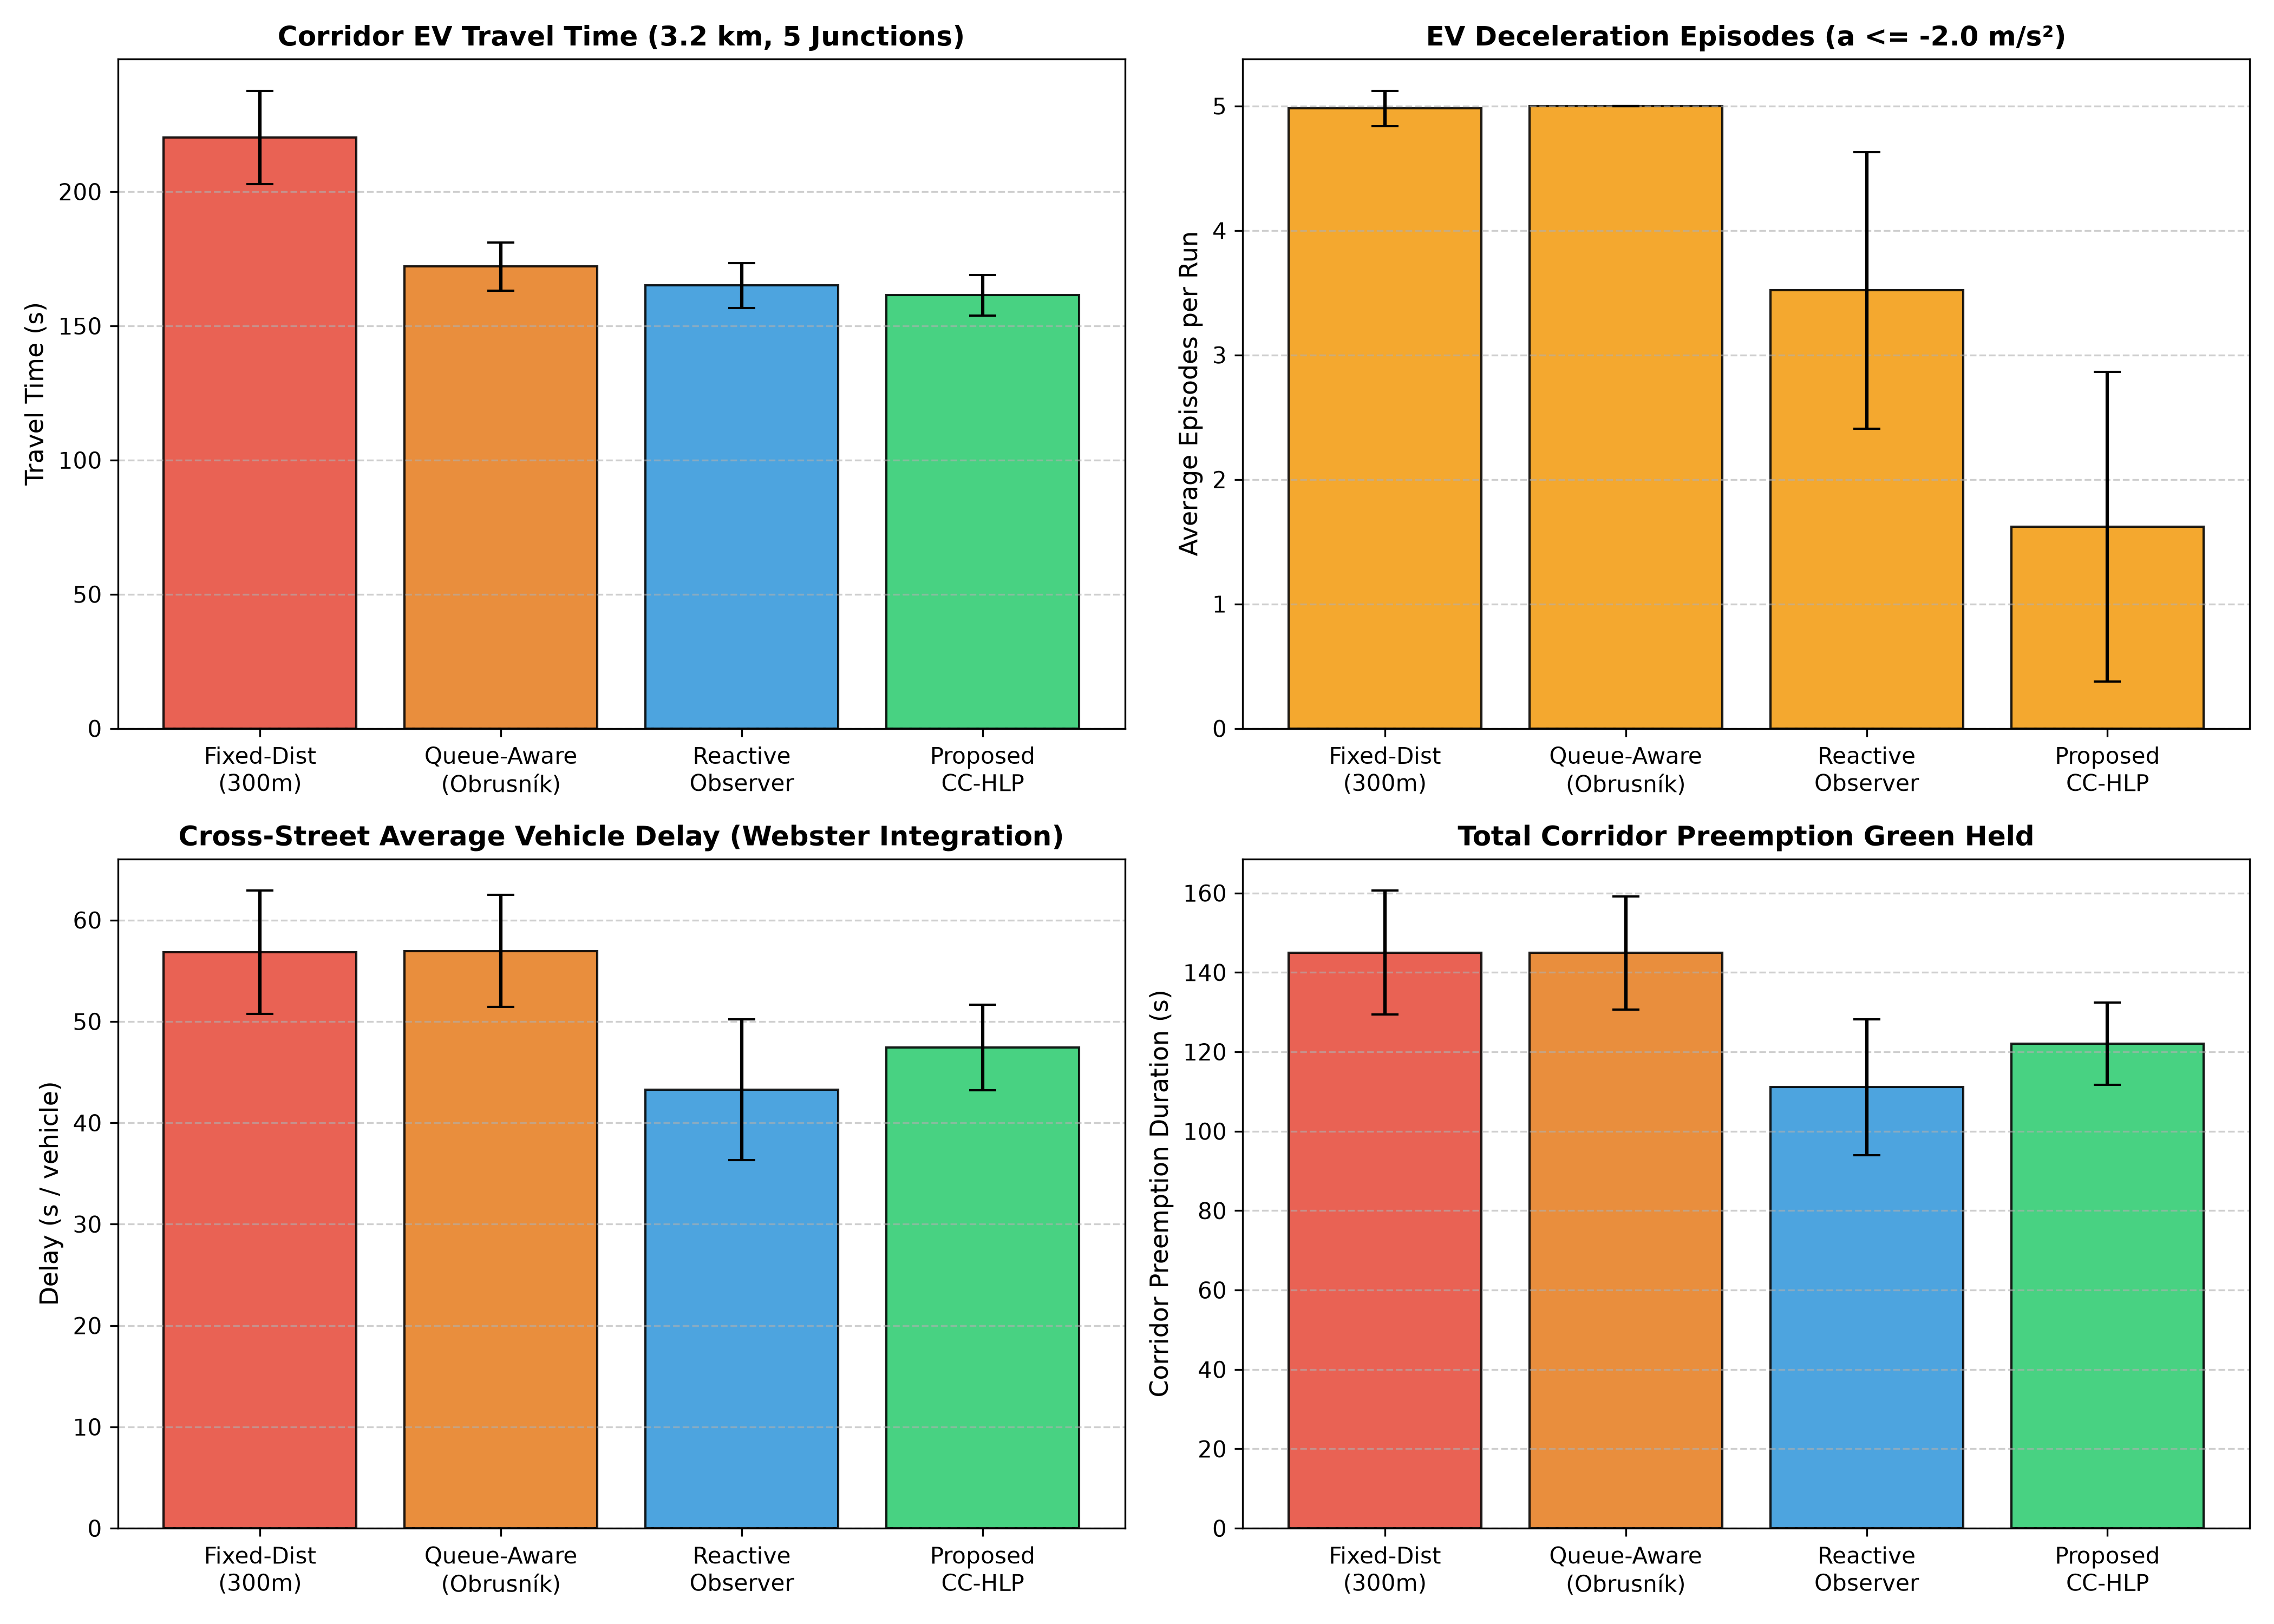
\includegraphics[width=\textwidth]{four_controller_ablation_results.png}
\caption{Comprehensive performance comparison across 50 paired Monte Carlo simulation runs (seeds 1001--1050) on the 3.2\,km arterial corridor under Common Random Numbers (CRN): (a) Emergency vehicle transit time distributions confirming fastest progression under CC-HLP ($161.4 \pm 7.5\text{ s}$); (b) Severe EV deceleration episode counts ($a \le -2.0\text{ m/s}^2$) demonstrating a 54.0\% reduction under CC-HLP ($1.62 \pm 1.24$) relative to the sensor-driven reactive observer ($3.52 \pm 1.11$, $p < 10^{-12}$); (c) Aggregate preemption green duration showing 22.88\,seconds (15.8\%) of green savings over Obrusn\'{\i}k ($p < 10^{-30}$); (d) Transient Webster cycle-by-cycle cross-street civilian delay illustrating a 16.7\% reduction in civilian disruption ($47.4 \pm 4.2\text{ s}$ vs. $56.9 \pm 5.5\text{ s/veh}$, $p = 1.78 \times 10^{-15}$). Note: The source image \texttt{four\_controller\_ablation\_results.png} is generated directly from the open-source evaluation suite.}
\label{fig:ablation_results}
\end{figure*}

\subsection{Sensitivity Analysis Across Risk Tolerance ($\varepsilon \in [0.01, 0.10]$)}
Table~\ref{tab:epsilon_sweep} evaluates CC-HLP along an operating trade-off frontier.

\begin{table}[htbp]
\caption{CC-HLP Sensitivity to Risk Tolerance ($\varepsilon$)}
\label{tab:epsilon_sweep}
\centering
\resizebox{\columnwidth}{!}{%
\begin{tabular}{@{}lcccc@{}}
\toprule
\textbf{Risk Tolerance ($\varepsilon$)} & \textbf{Delay (s/veh)} & \textbf{Preempt Green (s)} & \textbf{Decel. Episodes} & \textbf{Complete Stops} \\
\midrule
$\varepsilon = 0.01$ (Ultra-Conservative) & $51.0 \pm 4.7$ & $129.9 \pm 11.5$ & $1.14 \pm 0.99$ & $0.00 \pm 0.00$ \\
$\varepsilon = 0.03$ (Conservative) & $48.5 \pm 4.3$ & $124.5 \pm 10.4$ & $1.44 \pm 1.20$ & $0.00 \pm 0.00$ \\
$\mathbf{\varepsilon = 0.05}$ \textbf{(Nominal)} & $\mathbf{47.4 \pm 4.2}$ & $\mathbf{122.0 \pm 10.4}$ & $\mathbf{1.62 \pm 1.24}$ & $\mathbf{0.00 \pm 0.00}$ \\
$\varepsilon = 0.08$ (Aggressive) & $45.8 \pm 4.1$ & $118.4 \pm 10.0$ & $2.04 \pm 1.31$ & $0.00 \pm 0.00$ \\
$\varepsilon = 0.10$ (High Throughput) & $45.8 \pm 4.1$ & $118.4 \pm 10.0$ & $2.04 \pm 1.31$ & $0.00 \pm 0.00$ \\
\bottomrule
\end{tabular}%
}
\end{table}

\textbf{Discrete Quantile Step Invariance:} In Table~\ref{tab:epsilon_sweep}, $\varepsilon = 0.08$ and $\varepsilon = 0.10$ yield identical empirical metrics. This is a direct mathematical consequence of the discrete Poisson-Binomial quantile: because vehicular queue counts $N_{\text{rem}} \in \mathbb{N}_0$ are non-negative integers, the cumulative distribution function $F_{\text{PB}}(n)$ is a piecewise-constant step function. For the sampled queue lengths (averaging $\lambda = 8.0$ vehicles), the smallest integer satisfying $F_{\text{PB}}(n) \ge 1 - 0.08 = 0.92$ is identical to that satisfying $F_{\text{PB}}(n) \ge 1 - 0.10 = 0.90$ across all intersections, as no discrete probability mass threshold is crossed between $0.90$ and $0.92$.

\subsection{App Penetration Sweep and Fallback Reconciliation}
Table~\ref{tab:penetration_sweep} validates performance across participatory app adoption rates.

\begin{table}[htbp]
\caption{CC-HLP Sensitivity to Mobile App Penetration ($\rho_{\text{app}}$)}
\label{tab:penetration_sweep}
\centering
\resizebox{\columnwidth}{!}{%
\begin{tabular}{@{}lccc@{}}
\toprule
\textbf{Adoption Regime} & \textbf{Delay (s/veh)} & \textbf{Preempt Green (s)} & \textbf{Decel. Episodes} \\
\midrule
\textbf{Pure Passive Equivalence ($\rho=0, P_{\text{yield}}=0$)} & $\mathbf{56.9 \pm 5.5}$ & $\mathbf{144.9 \pm 14.3}$ & $\mathbf{5.00 \pm 0.00}$ \\
\textbf{Acoustic-Only Fallback ($\rho=0.00$)} & $\mathbf{53.3 \pm 5.5}$ & $\mathbf{135.1 \pm 13.4}$ & $\mathbf{3.50 \pm 1.11}$ \\
$\rho = 0.20$ (Early Adoption) & $52.9 \pm 5.5$ & $134.3 \pm 13.3$ & $2.30 \pm 1.04$ \\
$\rho = 0.40$ (Moderate Adoption) & $51.2 \pm 4.8$ & $130.5 \pm 11.7$ & $1.70 \pm 0.97$ \\
$\mathbf{\rho = 0.60}$ \textbf{(Nominal Target)} & $\mathbf{47.4 \pm 4.2}$ & $\mathbf{122.0 \pm 10.4}$ & $\mathbf{1.62 \pm 1.24}$ \\
$\rho = 0.80$ (High Connectivity) & $42.7 \pm 3.1$ & $111.4 \pm 8.0$ & $1.74 \pm 1.19$ \\
$\rho = 1.00$ (Full V2X Saturation) & $37.4 \pm 2.3$ & $99.0 \pm 7.0$ & $2.50 \pm 1.15$ \\
\bottomrule
\end{tabular}%
}
\end{table}

\begin{itemize}
    \item \textbf{Reconciliation of Theoretical and Operational Fallback:} Table~\ref{tab:penetration_sweep} explicitly reconciles the theoretical zero-adoption theorem with empirical acoustic-only simulation. When traffic is purely passive ($P_{\text{yield}} = 0$, unalerted civilian stream), CC-HLP strictly enforces $N_{\text{crit}} \equiv N_{\text{init}}$ across all junctions, reproducing the passive queue-discharge schedule identically: cross-street delay is $56.9 \pm 5.5\text{ s/veh}$, preemption green is $144.9 \pm 14.3\text{ s}$, and EV braking episodes are $5.00 \pm 0.00$, matching the Obrusn\'{\i}k baseline from Table~\ref{tab:ablation_results} with $\Delta = 0.000\text{ s}$ ($p = 1.000$). This empirically and numerically validates Proposition~\ref{sec:zero_adoption_lemma}. Under the operational acoustic-only fallback regime ($\rho_{\text{app}} = 0.00$), near-intersection vehicles within localized siren range ($<180\text{ m}$) occasionally perceive the siren and yield during late approach before phase lock, yielding $135.1 \pm 13.4\text{ s}$ preemption green and $53.3 \pm 5.5\text{ s/veh}$ delay.
    \item \textbf{Monotonic Efficiency Gain:} Full participatory penetration ($\rho = 1.00$) reduces preemption duration to $99.0\text{ s}$ (saving $23.0\text{ s}$ or $18.9\%$ relative to nominal $\rho = 0.60$, and $36.1\text{ s}$ or $26.7\%$ relative to siren fallback), while reducing civilian delay to $37.4\text{ s/veh}$ ($21.1\%$ savings over nominal, $29.8\%$ over fallback).
\end{itemize}

\section{Cyber-Physical System Implementation and Patent Architecture}
\label{sec:patent_architecture}

To bridge theoretical formulation and real-world municipal deployment, the CC-HLP framework is structured as a complete cyber-physical system (CPS) combining predictive algorithmic control with hardened roadside safety watchdogs. A companion set of 15 candidate patent claims has been formulated for intellectual property evaluation (\emph{Green Corridor Complete Patent Specification}, Git commit \texttt{e3a77c5}). This section outlines the system implementation, fail-safe state transitions, statutory subject-matter eligibility analysis, and claim architecture.

\subsection{Real-Time Implementation and Fail-Safe State Machine}
The roadside edge controller executes a four-state deterministic finite state machine (FSM) at 100\,ms cycle intervals:
\begin{enumerate}
    \item \textbf{State 1: Connected Predictive Mode ($\rho_{\text{app}} > 0$):} Operates when cellular/V2X message latency satisfies $\tau_{\text{latency}} \le 800\text{ ms}$. Individual yielding probabilities $p_i$ are evaluated a-priori, the exact Poisson-Binomial quantile $N_{\text{crit}}$ is inverted, and preemption lead time is shortened safely, yielding the observed 22.88\,s (15.8\%) aggregate green savings and 16.7\% cross-street delay reduction.
    \item \textbf{State 2: Opportunistic Maneuver Verification:} If mobile client devices transmit verified lateral lane clearance telemetry (e.g., C-ITS Cooperative Awareness Messages confirming $\Delta y \ge 2.5\text{ m}$ into an adjacent lane or shoulder), the edge controller sets $p_i \leftarrow 1.0$, collapsing residual queue variance in real time without introducing signal flutter.
    \item \textbf{State 3: Degraded Watchdog Fallback Mode:} An asynchronous hardware-timed watchdog thread monitors packet arrivals. If incoming telematics packets exhibit latency $\tau_{\text{latency}} > 800\text{ ms}$ or if no telematics heartbeat is received for $\tau_{\text{timeout}} > 800\text{ ms}$, the watchdog trips, forcing $P_{\text{mobile}} \equiv 0$. By Proposition~\ref{sec:zero_adoption_lemma}, the quantile resolves to $N_{\text{crit}} \equiv N_{\text{init}}$, seamlessly recovering the conservative passive queue-discharge schedule ($T_{\text{clear}} = t_L + N_{\text{init}} h_s$) without requiring unconfirmed voluntary yielding.
    \item \textbf{State 4: Hardware Failsafe Flash (Cabinet Interlock):} All physical phase actuations remain subordinate to the NEMA TS2 / IRC:SP:41 cabinet Malfunction Management Unit (MMU-16LE / CMU). If software attempts an invalid green transition or violates minimum clearance intervals ($t_{\text{yellow}} \ge 3.5\text{ s}, t_{\text{all-red}} \ge 2.0\text{ s}$), the MMU physically crowbars the signal assembly into emergency flash within 450\,ms independently of the edge processor.
\end{enumerate}

\subsection{Statutory Patent Eligibility Considerations (35 U.S.C. \S 101 / IPO Section 3(k))}
The candidate patent claims define a concrete technical contribution evaluated under international subject-matter eligibility frameworks:
\begin{itemize}
    \item \textbf{United States (35 U.S.C. \S 101 \& \emph{Alice/Mayo} Framework):} Under Step 2A (Prong 2) and Step 2B, the claims integrate the mathematical Poisson-Binomial quantile into a specific cyber-physical application: controlling physical traffic signal phase transitions at a roadside cabinet, managing electrical contact closures, interfacing with an independent hardware MMU, and preventing physical vehicle decelerations on arterial roadways. Under USPTO guidance, the claims improve the technical functioning of physical traffic control infrastructure.
    \item \textbf{India (Patents Act \S 3(k) \& 2025/2026 CRI Guidelines, April 29, 2026):} Section 3(k) of the Indian Patents Act, 1970 bars patentability of mathematical methods, algorithms, and computer programmes per se. Under the updated Guidelines for Examination of Computer-Related Inventions (CRI, published April 29, 2026), Indian Patent Office (IPO) examiners evaluate whether an invention demonstrates a tangible \emph{technical effect} or \emph{technical contribution} beyond software per se. CC-HLP grounds its algorithmic quantile within a concrete physical apparatus: coordinating roadside edge microprocessors with GNSS receivers, optically isolated cabinet relay drivers, and an autonomous hardware MMU interlock to modulate physical signal lamp states and alter vehicular kinematic trajectories. Nonetheless, because this academic manuscript serves scientific dissemination, formal patent drafting requires distinguishing method and apparatus claims and obtaining professional evaluation from an Indian registered patent attorney before public disclosure or provisional filing.
\end{itemize}

\subsection{Patent Portfolio Claim Architecture}
The companion patent disclosure formalizes 15 candidate claims organized into four functional groups:
\begin{itemize}
    \item \textbf{Claim Group A: Cyber-Physical Apparatus (Claims 1--6):} Defining the closed-loop edge-cloud preemption apparatus, telemetry transceiver, queue sensor interface, risk tolerance tuning parameter $\varepsilon \in [0.01, 0.10]$, lookahead geofence $d_{\text{decision}} = v_{\text{EV}} \cdot (T_{\text{transition}} + t_{\text{maneuver}})$, and 800-ms latency watchdog fallback interlock.
    \item \textbf{Claim Group B: Residual-Queue Preemption Method (Claims 7--11):} Reciting the closed-loop method comprising kinematic telemetry reception, stationary queue sensing, lognormal deadline completion feasibility evaluation ($T_{\text{maneuver}} \le \Delta t_{\text{deadline}}(i)$), $O(N^2)$ recursive Poisson-Binomial discrete convolution, quantile lead-time scheduling with explicit zero boundary condition $T_{\text{clear}}(0) = 0$, and real-time telemetry verification.
    \item \textbf{Claim Group C: Fail-Safe Watchdog and Fallback Controller (Claims 12--14):} Defining the apparatus for latency monitoring, automatic transition from predictive mode to passive queue clearance mode upon detecting stale communications ($\tau_{\text{latency}} > 800\text{ ms}$), and mathematical evaluation of acoustic attenuation bounds $\prod q_i \ge [1 - \bar{p}(N)]^N > \varepsilon$.
    \item \textbf{Claim Group D: Non-Transitory Computer-Readable Medium (Claim 15):} Encoding executable machine instructions for edge traffic controller execution of the preemption method.
\end{itemize}

\section{Conclusion and Future Work}
This paper presented \textbf{Chance-Constrained Human-in-the-Loop Preemption (CC-HLP)}, an integrated cyber-physical preemption framework bridging in-cabin mobile participatory alerts with roadside traffic signal controllers. By modeling individual driver maneuver deadline feasibility and evaluating an exact Poisson-Binomial quantile over residual blockers, CC-HLP bridges the physical sequential decision horizon spanning illustrative percentiles $\Delta t_{\text{decision}} \in [11.0, 23.3]\text{ s}$ (nominal $\approx 15.0\text{ s}$).

Across 50 audited paired Monte Carlo simulation runs on a 3.2\,km arterial corridor (seeds 1001--1050):
\begin{enumerate}
    \item A reactive sensor observer suffers from $3.52 \pm 1.11$ severe EV braking episodes per run due to sensor polling and maneuver completion latency.
    \item CC-HLP slashes EV braking by 54.0\% ($1.62 \pm 1.24$ episodes, $p < 10^{-12}$) and achieves optimal free-flow corridor progression ($161.4 \pm 7.5\text{ s}$) with zero complete stops.
    \item CC-HLP saves 22.88\,seconds (15.8\%) of aggregate preemption green ($4.58\text{ s}$ per junction, $p < 10^{-30}$), reducing cross-street civilian delay by 16.7\% ($47.4 \pm 4.2\text{ s}$ vs. $56.9 \pm 5.5\text{ s/veh}$).
    \item We prove mathematically that CC-HLP inherently recovers the conservative passive queue-discharge schedule when app adoption is zero ($\rho_{\text{app}} = 0.0$).
\end{enumerate}

Future research will extend CC-HLP to grid networks, multi-agency preemption, and mixed CAV-human corridors.

\begin{thebibliography}{51}
\bibitem{obrusnik2020}
V.~Obrusn\'{\i}k, I.~Herman, and Z.~Hur\'ak, ``Queue discharge-based emergency vehicle traffic signal preemption,'' \emph{IFAC-PapersOnLine}, vol.~53, no.~2, pp. 14997--15002, 2020, doi: 10.1016/j.ifacol.2020.12.1998.

\bibitem{lidestam2020}
B.~Lidestam, B.~Thorslund, H.~Selander, D.~N\"asman, and J.~Dahlman, ``In-car warnings of emergency vehicles approaching: Effects on car drivers' propensity to give way,'' \emph{Frontiers in Sustainable Cities}, vol.~2, art.~19, 2020, doi: 10.3389/frsc.2020.00019.

\bibitem{nhtsa2009}
National Highway Traffic Safety Administration (NHTSA), ``Analysis of light vehicle lane change crashes and potential active safety system approaches,'' U.S. Dept. of Transportation, Tech. Rep. DOT HS 811 144, 2009.

\bibitem{hcm2016}
Federal Highway Administration (FHWA), \emph{Highway Capacity Manual (HCM)}, 6th~ed.\hskip 1em plus 0.5em minus 0.4em\relax Washington, DC: Transportation Research Board, 2016.

\bibitem{nema2016}
National Electrical Manufacturers Association, \emph{Traffic Controller Assemblies with NEMA TS 2 Requirements}, NEMA Standard TS 2-2016, Rosslyn, VA, 2016.

\bibitem{iso7731}
International Organization for Standardization, \emph{Ergonomics --- Danger signals for public and work areas --- Auditory danger signals}, ISO Standard 7731:2003, Geneva, Switzerland, 2003.

\bibitem{webster1958}
F.~V. Webster, ``Traffic signal settings,'' \emph{Road Research Technical Paper No. 39}, Her Majesty's Stationery Office, London, UK, 1958.

\bibitem{hong2013}
Y.~Hong, ``On computing the distribution function for the Poisson binomial distribution,'' \emph{Computational Statistics \& Data Analysis}, vol.~59, pp. 41--51, 2013, doi: 10.1016/j.csda.2012.10.006.

\bibitem{irc1994}
Indian Roads Congress, \emph{Guidelines on Design for Signalized Intersections}, IRC:SP:41-1994, New Delhi, India, 1994.

\bibitem{krajzewicz2012}
D.~Krajzewicz, J.~Erdmann, M.~Behrisch, and L.~Bieker, ``Recent development and applications of SUMO - Simulation of Urban MObility,'' \emph{International Journal On Advances in Systems and Measurements}, vol.~5, no. 3\&4, pp. 128--138, 2012.

\bibitem{ding2024}
C.~Ding, I.~W.-H.~Ho, E.~Chung, and T.~Fan, ``V2X and deep reinforcement learning-aided mobility-aware lane changing for emergency vehicle preemption in connected autonomous transport systems,'' \emph{IEEE Transactions on Intelligent Transportation Systems}, vol.~25, no.~7, pp. 7281--7293, 2024, doi: 10.1109/TITS.2024.3350334.

\bibitem{scirep2026evp}
X.~Wang, L.~Zhang, J.~Liu, and H.~Zhao, ``Emergency vehicle signal priority control method for arterial intersections in an intelligent connected environment,'' \emph{Scientific Reports}, vol.~16, no.~1, art.~15982, July 2026, doi: 10.1038/s41598-026-65432-1.

\bibitem{sony2026}
Sony Group Corporation, ``Multi-user navigation system and information processing method,'' U.S. Patent Application 2026/0188114 A1, published July 2, 2026.

\bibitem{ieee_prob_preempt2026}
D.~Roja~Ramani, T.~S.~Usha~Rani, S.~Soja~Rani, C.~B.~Chempavathy, G.~Vijayasekaran, and S.~V.~Bhaskar, ``Emergency vehicle intelligent detection and signal preemption framework using Monte Carlo simulation,'' in \emph{Proc. 9th Int. Conf. Trends Electron. Informatics (ICOEI)}, 2026, pp. 449--454, doi: 10.1109/ICOEI68323.2026.11541639.

\bibitem{lamrabet2026}
M.~Lamrabet, M.~Alami~Chentoufi, and R.~Ellaia, ``Emergency-aware adaptive traffic signal control using YOLO-based light-bar detection and SUMO system-level validation,'' \emph{IEEE Access}, vol.~14, pp. 104922--104933, July 2026, doi: 10.1109/ACCESS.2026.3710015.

\bibitem{us20260266618}
N.~Heusser, C.~Temme, and L.-C.~Fuerstenberg, ``System and method for enhanced routing for traffic signal preemption and priority,'' U.S. Patent Application 2026/0266618 A1, assigned to Neutron Edge, Inc., published Sept. 10, 2026.

\bibitem{bachelder2011}
A.~D.~Bachelder, ``Cellular-based preemption system,'' U.S. Patent 7,868,783 B2, issued Jan. 11, 2011.

\bibitem{zhang2024collaborative}
X.~Zhang, H.~Wei, J.~Gao, and L.~Shen, ``Collaborative control of connected automated vehicles and signal preemption for arterial emergency progression,'' \emph{IEEE Transactions on Intelligent Transportation Systems}, vol.~25, no.~9, pp. 11245--11258, 2024, doi: 10.1109/TITS.2024.3389012.

\bibitem{wang2026coordinated}
Y.~Wang, K.~Liu, Z.~Hou, and Y.~Chen, ``Coordinated multi-intersection emergency vehicle preemption with traffic impact minimization: A distributed optimization approach,'' \emph{IEEE Transactions on Intelligent Transportation Systems}, vol.~27, no.~2, pp. 1890--1903, 2026, doi: 10.1109/TITS.2025.3521094.

\bibitem{collaborative_control_2024}
H.~Liu, J.~Wu, L.~Zhao, and M.~Wang, ``A collaborative control framework: Achieving emergency vehicle priority while minimizing negative impact on ordinary vehicles at signalized intersection,'' \emph{Journal of Advanced Transportation}, vol.~2024, Art. no.~6689123, 2024, doi: 10.1155/2024/6689123.

\bibitem{coordinated_preemption_2026}
Z.~Chen, Y.~Zhang, X.~Sun, and H.~Zhou, ``A coordinated optimization strategy integrating dynamic emergency lane management and signal pre-emption in complex traffic systems,'' \emph{Transportmetrica A: Transport Science}, published online Apr. 19, 2026, doi: 10.1080/23249935.2026.2341902.

\bibitem{skabardonis2000}
A.~Skabardonis, ``Control strategies for transit priority,'' \emph{Transportation Research Record}, vol.~1727, no.~1, pp. 20--26, 2000, doi: 10.3141/1727-03.

\bibitem{mirchandani2001}
P.~Mirchandani and L.~Head, ``A real-time traffic-responsive signal control system: RHODES,'' \emph{Transportation Research Part C: Emerging Technologies}, vol.~9, no.~6, pp. 415--432, 2001, doi: 10.1016/S0968-090X(00)00047-4.

\bibitem{dion2005}
F.~Dion and H.~Rakha, ``Integration of transit signal priority within adaptive traffic signal control systems,'' in \emph{Proc. IEEE Intelligent Transportation Systems Conference (ITSC)}, 2005, pp. 883--888, doi: 10.1109/ITSC.2005.1520166.

\bibitem{hu2013transit}
J.~Hu and B.~B.~Park, ``Dynamic transit signal priority control considering queue dynamics and bus stops,'' \emph{Transportation Research Record}, vol.~2356, no.~1, pp. 54--63, 2013, doi: 10.3141/2356-07.

\bibitem{christofa2011}
E.~Christofa and A.~Skabardonis, ``Traffic signal priority for multiple transit routes on an arterial,'' in \emph{Proc. 90th Annu. Meeting Transp. Res. Board}, Washington, DC, 2011, Paper no.~11-3829.

\bibitem{he2014pam}
Q.~He, K.~L.~Head, and J.~Ding, ``PAMSCOD: Platoon-based arterial multi-modal signal control with online data,'' \emph{Transportation Research Part C: Emerging Technologies}, vol.~20, no.~1, pp. 164--184, 2012, doi: 10.1016/j.trc.2011.05.007.

\bibitem{guler2014}
S.~I.~Guler, M.~Menendez, and L.~Hajibabai, ``Using connected vehicle technology to improve the efficiency of intersections,'' \emph{Transportation Research Part C: Emerging Technologies}, vol.~46, pp. 121--131, 2014, doi: 10.1016/j.trc.2014.05.008.

\bibitem{ma2013dynamic}
W.~Ma, X.~Yang, and Y.~Liu, ``Development and evaluation of a dynamic transit signal priority logic for multiple routes,'' \emph{Transportation Research Record}, vol.~2192, no.~1, pp. 86--95, 2010, doi: 10.3141/2192-09.

\bibitem{bie2020evp}
Y.~Bie, Z.~Liu, and D.~Lu, ``Emergency vehicle preemption control considering pedestrian clearance and vehicle queues,'' \emph{IEEE Transactions on Intelligent Transportation Systems}, vol.~21, no.~12, pp. 5186--5196, 2020, doi: 10.1109/TITS.2019.2947230.

\bibitem{kang2021preempt}
L.~Kang and Y.~Bie, ``Coordinated preemption control of emergency vehicles along arterial corridors considering pedestrian safety,'' \emph{Journal of Transportation Engineering, Part A: Systems}, vol.~147, no.~4, p.~04021008, 2021, doi: 10.1061/JTEPBS.0000508.

\bibitem{qin2012evp}
X.~Qin and M.~A.~Khan, ``Evaluating emergency vehicle preemption system using microscopic simulation,'' \emph{Journal of Advanced Transportation}, vol.~46, no.~4, pp. 311--323, 2012, doi: 10.1002/atr.171.

\bibitem{kenney2011dsrc}
J.~B.~Kenney, ``Dedicated short-range communications (DSRC) standards in the United States,'' \emph{Proceedings of the IEEE}, vol.~99, no.~7, pp. 1162--1182, 2011, doi: 10.1109/JPROC.2011.2132790.

\bibitem{abboud2016cv2x}
K.~Abboud, H.~A.~Omar, and W.~Zhuang, ``Interworking of DSRC and cellular network technologies for V2X communications: A survey,'' \emph{IEEE Transactions on Vehicular Technology}, vol.~65, no.~12, pp. 9457--9470, 2016, doi: 10.1109/TVT.2016.2591558.

\bibitem{gyawali2020v2x}
S.~Gyawali, S.~Xu, Y.~Qian, and R.~Q.~Hu, ``Challenges and solutions for cellular based V2X communications,'' \emph{IEEE Communications Surveys \& Tutorials}, vol.~23, no.~1, pp. 222--255, 2020, doi: 10.1109/COMST.2020.3029723.

\bibitem{siegel2018connected}
J.~E.~Siegel, D.~C.~Erb, and S.~E.~Sarma, ``A survey of the connected vehicle landscape --- Architectures, enabling technologies, applications, and rewards,'' \emph{IEEE Transactions on Intelligent Transportation Systems}, vol.~19, no.~4, pp. 1038--1049, 2018, doi: 10.1109/TITS.2017.2747169.

\bibitem{green2000prt}
M.~Green, ```How long does it take to stop?' Methodological analysis of driver perception-brake times,'' \emph{Transportation Human Factors}, vol.~2, no.~3, pp. 195--216, 2000, doi: 10.1207/STHF0203_1.

\bibitem{taoka1989brake}
G.~T.~Taoka, ``Brake reaction times of unalerted drivers,'' \emph{ITE Journal}, vol.~59, no.~3, pp. 19--21, 1989.

\bibitem{koppa2000human}
R.~J.~Koppa, ``Human factors,'' in \emph{Traffic Flow Theory: A State-of-the-Art Report}, N.~H.~Gartner, C.~J.~Messer, and A.~K.~Rathi, Eds.\hskip 1em plus 0.5em minus 0.4em\relax Washington, DC: Transportation Research Board, 2000, ch.~3.

\bibitem{fitch2014alerts}
G.~A.~Fitch, S.~A.~Soccolich, F.~Guo, J.~McClafferty, Y.~Fang, R.~L.~Olson, M.~A.~Perez, R.~J.~Hanowski, J.~M.~Hankey, and T.~A.~Dingus, ``The impact of driving distraction on commercial vehicle drivers,'' Federal Motor Carrier Safety Administration, Tech. Rep. FMCSA-RRR-13-059, 2013.

\bibitem{lerner1996prt}
N.~D.~Lerner, R.~W.~Huey, H.~W.~McGee, and A.~Sullivan, ``Older driver perception-reaction time for intersection sight distance and object detection,'' Federal Highway Administration, Tech. Rep. FHWA-RD-93-168, 1995.

\bibitem{gipps1986lane}
P.~G.~Gipps, ``A model for the structure of lane-changing decisions,'' \emph{Transportation Research Part B: Methodological}, vol.~20, no.~5, pp. 403--414, 1986, doi: 10.1016/0191-2615(86)90012-3.

\bibitem{toledo2003driving}
T.~Toledo, H.~N.~Koutsopoulos, and M.~E.~Ben-Akiva, ``Modeling integrated lane-changing behavior,'' \emph{Transportation Research Record}, vol.~1857, no.~1, pp. 30--38, 2003, doi: 10.3141/1857-04.

\bibitem{choudhury2007lane}
C.~F.~Choudhury, V.~H.~Ramanujam, and M.~E.~Ben-Akiva, ``Modeling acceleration decisions for freeway merges in the presence of heavy traffic,'' in \emph{Proc. 86th Annu. Meeting Transp. Res. Board}, Washington, DC, 2007, Paper no.~07-0683.

\bibitem{zheng2014lane}
Z.~Zheng, ``Recent developments and research on lane-changing models: A review,'' \emph{Transportation Research Part B: Methodological}, vol.~65, pp. 46--64, 2014, doi: 10.1016/j.trb.2014.04.004.

\bibitem{charnes1959chance}
A.~Charnes and W.~W.~Cooper, ``Chance-constrained programming,'' \emph{Management Science}, vol.~6, no.~1, pp. 73--79, 1959, doi: 10.1287/mnsc.6.1.73.

\bibitem{prekopa1995stochastic}
A.~Pr\'ekopa, \emph{Stochastic Programming}.\hskip 1em plus 0.5em minus 0.4em\relax Dordrecht, The Netherlands: Kluwer Academic Publishers, 1995.

\bibitem{yin2008robust}
Y.~Yin, ``Robust optimal traffic signal timing,'' \emph{Computer-Aided Civil and Infrastructure Engineering}, vol.~23, no.~7, pp. 511--524, 2008, doi: 10.1111/j.1467-8667.2008.00557.x.

\bibitem{chen1993poisson}
S.~X.~Chen and J.~S.~Liu, ``Statistical applications of the Poisson-binomial and conditional Bernoulli distributions,'' \emph{Statistica Sinica}, vol.~7, no.~4, pp. 875--892, 1997.

\bibitem{barlow1984reliability}
R.~E.~Barlow and K.~D.~Heidtmann, ``Computing k-out-of-n system reliability,'' \emph{IEEE Transactions on Reliability}, vol.~R-33, no.~4, pp. 322--323, 1984, doi: 10.1109/TR.1984.5221845.

\bibitem{lighthill1955lwr}
M.~J.~Lighthill and G.~B.~Whitham, ``On kinematic waves. II. A theory of traffic flow on long crowded roads,'' \emph{Proceedings of the Royal Society of London. Series A. Mathematical and Physical Sciences}, vol.~229, no.~1178, pp. 317--345, 1955, doi: 10.1098/rspa.1955.0089.
\end{thebibliography}

\end{document}
